\documentclass[a4paper, 12pt]{report}

\usepackage[a4paper,bindingoffset=0.2in,%
            left=0.5in,right=0.7in,top=0.7in,bottom=1.25in,%
            footskip=0.5in]{geometry}
\usepackage{amsmath, amssymb, amsfonts, amsthm, mathtools}
\usepackage{bm}
\usepackage{graphicx}
\usepackage{float}
\usepackage{slashbox}
\usepackage{listings}
\usepackage{commath}
\usepackage{tikz}
\usepackage[hidelinks]{hyperref}
\usepackage{xcolor}
\usetikzlibrary{matrix,calc}

\setlength{\parindent}{0pt}

\title{
	{\huge\bf Summer of Science 2020} \\
	[1cm]
	\textit{Final Report} \\
	[1cm]
	{\LARGE\scshape An Overview of Machine Learning, \\ Neural Networks, and Deep Learning} \\
	\begin{figure}[H]
	\centering
	\includegraphics[width=0.45\textwidth]{Machine-Learning}
	\end{figure}
}
\author{
	Ankit Kumar Misra \\
	Roll No. 190050020 \\
	Computer Science and Engineering \\
	IIT Bombay\\
	[1cm]
	Mentor: Soumya Chatterjee\\
	[1cm]
}
\date{\today}

\begin{document}

\pagenumbering{roman}

\maketitle

\chapter*{Introduction}
This report was written by me as part of my Summer of Science (SoS) project, organized by the Maths and Physics (MnP) Club, IIT Bombay, in the summer of 2020. I used this opportunity to dive into the world of machine learning and deep learning. This report consists of summaries of just about everything I learned throughout the project, including descriptions of various machine learning algorithms as I understood them, with special emphasis on neural networks and deep learning algorithms.\\
\break
This project has been an enlightening experience. Through this project, I've developed a great interest in learning algorithms, and in the future, I would like to get deeper into the more rigorous mathematics and statistics governing the algorithms I've learned about.\\
\break
I thank the MnP club, and my mentor Soumya Chatterjee, for the memorable summer experience with SoS 2020, and I hope you enjoy reading my report! Any feedback or suggestions are welcome at my email address: \textcolor{blue}{\href{mailto:ankitkumarmisra2001@gmail.com}{ankitkumarmisra2001@gmail.com}}.

\vspace{2.5cm}

\section*{Resources Used}
\vspace{0.7cm}
\begin{enumerate}
\item Andrew Ng's `Machine Learning' course on Coursera, by Stanford University
\item Andrew Ng's `Deep Learning Specialization' on Coursera, by deeplearning.ai
\item Online course material for Stanford University's CS231n course, titled `Convolutional Neural Networks for Visual Recognition'
\item `Deep Learning with Python' by Fran\c{c}ois Chollet
\item Various other online resources
\item Images from several online sources, acquired through Google Images
\end{enumerate}

\vspace*{\fill}

\newpage

\tableofcontents

\newpage

\pagenumbering{arabic}

\topskip0pt
\vspace*{\fill}
\begin{center}
{\huge\scshape Part I \\\vspace{1cm} Machine Learning}
\end{center}
\vspace*{\fill}

\newpage

\chapter{What is Machine Learning?}
The term \textit{machine learning} was coined by Arthur Samuel in 1959. He defined it as the field of study that gives computers the ability to learn without being explicitly programmed. \\
\break
In 1998, Tom Mitchell came up with a much more formal definition of a machine learning algorithm: \\
\textit{A computer program is said to learn from an experience E with respect to some task T and some performance measure P, if its performance on T, as measured by P, improves with experience E.} \\
\break
The main categories of machine learning algorithms are:
\begin{enumerate}
\item Supervised Learning
\item Unsupervised Learning
\item Reinforcement Learning
\end{enumerate}

\section{Supervised Learning}
Supervised learning algorithms are used when each training example in the training data consists of input feature values as well as the corresponding desired outputs. Thus, the algorithm is given the 'right answers' for the training inputs. Using a predefined cost function, the algorithm tries to generate a function that best fits this training data, and later uses this function to predict outputs for unseen inputs, that were not part of the training data. Supervised learning problems are of two types:
\begin{enumerate}
\item \textit{Regression}: These problems require the machine learning model to predict a continuous valued output; e.g., a housing price prediction problem is a regression task, since prices can take continuous values.
\item \textit{Classification}: These problems require the machine learning model to predict a discrete valued output; e.g., a problem which requires us to predict whether certain cancer tumors are benign or malignant is a classification task, since the output can take only two values; a tumor is either benign or malignant.
\end{enumerate}

\section{Unsupervised Learning}
Unsupervised learning algorithms are used to find structure in unlabeled and unclassified datasets that contains only inputs. The algorithm clusters data points; i.e., it assigns a set of observations into subsets (clusters) so that observations within the same cluster is similar, while observations from different clusters are dissimilar. Unsupervised learning algorithms are used in applications such as grouping similar news articles from different sources, social media analysis, market segmentation, and even astronomical data analysis.

\section{Reinforcement Learning}
Reinforcement learning algorithms are concerned with what actions a software agent should take in an environment in order to maximize a notion of cumulative reward. Owing to this generality, reinforcement learning algorithms are used in widely varying fields. The environment is represented as a Markov Decision Process, and the algorithm tries to take decisions based on its previous experiences in similar environments, thus attempting to maximize its reward.


\chapter{Linear Regression}
Linear regression is a supervised machine learning regression algorithm which, given a training dataset along with the corresponding continuous valued labels, determines the straight line function which best fits the training data. Thus, it assumes a linear function for the task and optimizes the function's parameters to fit the training data.
\vspace{1cm}
\hrule
\begin{center}
\textbf{NOTATION} \\
[8mm]
\begin{tabular}{p{1.8cm}p{9cm}}
$m$ & the number of instances in the dataset\\
[4mm]
$\bm{x^{\left(i\right)}}$ & the vector of all feature values (excluding the label) of the $i^{th}$ instance in the dataset\\
[4mm]
$y^{\left(i\right)}$ & the label (desired/expected output value) of the $i^{th}$ instance in the dataset \\
[4mm]
$\bm{x_j}$ & the vector of values from all data instances corresponding to the $j^{th}$ feature in the dataset\\
[4mm]
$x^{\left(i\right)}_j$ & the value of the $j^{th}$ feature in the $i^{th}$ instance of the dataset \\
[4mm]
$\bm{X}$ & the entire dataset (excluding labels) \\
[4mm]
$\bm{y}$ & the vector of all labels for the dataset \\
[4mm]
${\theta}_j$ & the parameter of the regression model which corresponds to the $j^{th}$ feature in the dataset \\
[4mm]
$\bm{\theta}$ & the vector of all parameters of the linear regression model \\
[4mm]
$h_{\theta}\left(\bm{x^{\left(i\right)}}\right)$ & the predicted label (output value) for the $i^{th}$ training instance
\end{tabular}
\end{center}
\hrule

\section{Hypothesis Function}
In linear regression tasks, the hypothesis function for an input data instance $\bm{x}$ having $n$ features and parameter vector $\bm{\theta}$ is given by:
\begin{align*}
h_{\theta}\left(\bm{x}\right) = \bm{\theta}^T\bm{x} = \theta_0x_0 + \theta_1x_1 + \theta_2x_2 + ... + \theta_nx_n
\end{align*}
Here, $x_0$ is always equal to 1, and $\theta_0$ is called the \textit{bias term}. It can be thought of as the intercept parameter. Therefore, any linear regression task is effectively a problem of analyzing the given training dataset and figuring out the best possible parameter vector which achieves the maximum accuracy among all possible parameter vectors. This is where the cost function comes in.

\begin{figure}[H]
\centering
\includegraphics[width=0.8\textwidth]{linear_regression}
\caption{Linear regression}
\end{figure}

\section{Cost Function}
In a machine learning algorithm, the cost function is used to determine the most accurate set of parameters which fits the training dataset. It provides a measure of the inaccuracy of the machine learning model, and the best possible parameters are determined by minimizing the cost function, using various methods. In linear regression tasks, the most commonly used cost function is:
\begin{align*}
J\left(\bm{\theta}\right) = \dfrac{1}{2m}\sum_{i=1}^{m}\left(h_{\theta}\left(\bm{x^{\left(i\right)}}\right)-y^{\left(i\right)}\right)^2 = \dfrac{1}{2m}\sum_{i=1}^{m}\left(\bm{\theta}^T\bm{x^{\left(i\right)}}-y^{\left(i\right)}\right)^2
\end{align*}
The linear regression model attempts to optimize this cost function, i.e., it calculates the parameters that minimize it. Several methods are available for this optimization, such as batch gradient descent, stochastic gradient descent, mini-batch gradient descent, and the method of normal equations.

\section{Gradient Descent}
The method of gradient descent first assumes a totally random parameter vector, and then moves towards the optimal parameters step by step. During each such step, the gradient of the cost function at the current parameter vector is computed, and a multiple of the gradient is subtracted from the parameter vector, so as to always keep moving along the direction of fastest descent. Note that we have to be careful with this method, since gradient descent moves towards a local minimum, and may never reach the global minimum.
The mathematical formulation for each step of gradient descent is as follows:
\begin{align*}
\bm{\theta}_{\text{new}} = \bm{\theta} - \alpha
\begin{pmatrix}
\dfrac{\partial}{\partial \theta_0}J\left(\bm{\theta}\right) \\
\dfrac{\partial}{\partial \theta_1}J\left(\bm{\theta}\right) \\
\vdots \\
\dfrac{\partial}{\partial \theta_n}J\left(\bm{\theta}\right) \\
\end{pmatrix}
= \bm{\theta} - \dfrac{\alpha}{m}
\begin{pmatrix}
\sum_{i=1}^{m}\left(h_{\theta}\left(\bm{x^{\left(i\right)}}\right)-y^{\left(i\right)}\right)x_0^{\left(i\right)} \\
\sum_{i=1}^{m}\left(h_{\theta}\left(\bm{x^{\left(i\right)}}\right)-y^{\left(i\right)}\right)x_1^{\left(i\right)} \\
\vdots \\
\sum_{i=1}^{m}\left(h_{\theta}\left(\bm{x^{\left(i\right)}}\right)-y^{\left(i\right)}\right)x_n^{\left(i\right)} \\
\end{pmatrix}
\end{align*}
\begin{align*}
\implies \bm{\theta}_{\text{new}} = \bm{\theta} - \dfrac{\alpha}{m}\sum_{i=1}^{m}\left(h_{\theta}\left(\bm{x^{\left(i\right)}}\right)-y^{\left(i\right)}\right)\bm{x^{\left(i\right)}} = \bm{\theta} - \dfrac{\alpha}{m}\bm{X}^T\left(\bm{X\theta} - \bm{y}\right)
\end{align*}
This formula is used for a method called batch gradient descent, where the entire dataset is considered in every single iteration, thus slowing down the training. To speed up the process, we can use stochastic gradient descent (one randomly selected instance in every iteration) or mini-batch gradient descent (a randomly selected subset of the dataset in every iteration).
\begin{figure}[H]
\centering
\includegraphics[width=1\textwidth]{gradient_descent}
\caption{Movement towards lower cost function values using gradient descent. For the sake of making visualization possible, this figure considers a dataset consisting of only two features, the corresponding parameters being $\theta_0$ and $\theta_1$.}
\end{figure}

\section{Normal Equations}
The normal equations method gives us a direct formula to calculate the optimized vector of parameters:
\begin{align*}
\bm{\theta} = \left(\bm{X}^T\bm{X}\right)^{-1}\bm{X}^T\bm{y}
\end{align*}
Although this gives us a direct method to obtain the answer in just one step, there is one major demerit. The matrix $\bm{X}^T\bm{X}$ is a square matrix having order equal to the number of instances in the dataset, and this makes inverse calculation computationally very expensive for larger datasets. The complexity of matrix inversion algorithms for an $n\times n$ matrix range from nearly $O(n^{2.37})$ to $O(n^3)$, and this large complexity is the main drawback for this method. Thus, gradient descent is preferred for datasets with more than $10,000$ data instances, whereas the normal equations method may be used for smaller datasets.

\section{Polynomial Regression}
Although polynomial regression is different from linear regression, a polynomial regression task can be reduced to a linear regression task by simply adding more features, formed by multiplication of powers of the existing features (according to the degree of polynomial regression), and then applying ordinary linear regression with all the features. Some datasets are better fit by polynomial functions than linear functions, and thus, a higher degree polynomial is often a better solution for the problem, as compared to a linear best fit.
\begin{figure}[H]
\centering
\includegraphics[width=0.6\textwidth]{polynomial_regression}
\caption{Polynomial regression}
\end{figure}

\newpage

\chapter{Logistic Regression}
Logistic regression is (quite confusingly, since it has the word \textit{regression}) a classification algorithm, under supervised learning. Given a training dataset along with the corresponding discrete valued labels, it determines a function to fit the dataset. The working principles of this algorithm are somewhat similar to those of linear regression. As for class representation, in a binary classification task, there is one scalar label for each data instance, which contains either 0 or 1, whereas in multiclass classification, the label is expressed as a one-hot encoded vector, wherein the index numbering equal to the correct class number has value 1 and all other indices have value 0. We discuss binary classification first.

\section{Hypothesis Function}
The hypothesis function in this case forces the weighted sum of feature values into the interval $\left[0, 1\right]$. This number represents the predicted probability of that instance having a label of 1. The hypothesis function is usually written as:
\begin{align*}
h_{\theta}\left(\bm{x}\right) = g\left(\bm{\theta}^T\bm{x}\right) \\
\text{where } \hspace{2mm} g\left(z\right) = \dfrac{1}{1+e^{-z}} \\
\therefore \hspace{2mm} h_{\theta}\left(\bm{x}\right) = \dfrac{1}{1+e^{-\bm{\theta}^T\bm{x}}}
\end{align*}
Using this probability vector, we predict the label as:
\begin{align*}
y =
\begin{cases}
1 & h_{\theta}\left(\bm{x}\right) \geq 0.5 \\
0 & h_{\theta}\left(\bm{x}\right) < 0.5
\end{cases}
\end{align*}
The above function $g\left(z\right)$ is called the sigmoid function. Also, the threshold here is 0.5, but in some special cases, where one out of precision or recall (later) is more important than the other, the threshold value can be changed to obtain better results.
\begin{figure}[H]
\centering
\includegraphics[width=0.6\textwidth]{sigmoid_graph}
\caption{Sigmoid function}
\end{figure}

\section{Decision Boundary}
It is clear from the graph of the sigmoid function, that it is an increasing function, and it takes a value of 0.5 at $z = 0$. Thus, we predict label:
\begin{align*}
y =
\begin{cases}
1 \text{ if } \bm{\theta}^T\bm{x} \geq 0 \\
0 \text{ if } \bm{\theta}^T\bm{x} < 0
\end{cases}
\end{align*}
This allows us to think of the classification in terms of a decision boundary. This boundary has the equation:
\begin{align*}
\theta_0 + \theta_1x_1 + \theta_2x_2 + ... + \theta_nx_n = 0
\end{align*}
The region where the above quantity is positive is the label 1 region, whereas the remaining region is the label 0 region.

\section{Cost Function}
In logistic regression, the cross-entropy cost function is used:
\begin{align*}
J\left(\bm{\theta}\right) = -\dfrac{1}{m}\sum_{i=1}^{m}\left[y^{\left(i\right)}\log h_{\theta}\left(\bm{x^{\left(i\right)}}\right) + \left(1 - y^{\left(i\right)}\right)\log \left(1 - h_{\theta}\left(\bm{x^{\left(i\right)}}\right)\right)\right]
\end{align*}
It is clear that the above function adds larger errors for larger deviations in the probability from the true labels. As in linear regression, the cost function is minimized using gradient descent (batch/stochastic/mini-batch). There is no normal equations method here.

\section{Gradient Descent}
As in linear regression, gradient descent is implemented by subtracting a multiple of the gradient of the cost function from the parameter vector at each step:
\begin{align*}
\bm{\theta}_{\text{new}} = \bm{\theta} - \alpha
\begin{pmatrix}
\dfrac{\partial}{\partial \theta_0}J\left(\bm{\theta}\right) \\
\dfrac{\partial}{\partial \theta_1}J\left(\bm{\theta}\right) \\
\vdots \\
\dfrac{\partial}{\partial \theta_n}J\left(\bm{\theta}\right) \\
\end{pmatrix}
= \bm{\theta} - \dfrac{\alpha}{m}\sum_{i=1}^{m}\left(h_{\theta}\left(\bm{x^{\left(i\right)}}\right)-y^{\left(i\right)}\right)\bm{x^{\left(i\right)}}
\end{align*}
As can be seen, the gradient expression turns out to be somewhat similar to that in linear regression.

\section{Multiclass Classification}
For multiclass classification, the one-vs-rest algorithm is used. In this method, the probability that an instance belongs to class $i$ is calculated for each class $i$, by creating several classifiers (number of classifiers equals the number of classes) and then training each classifier separately. For label prediction, the class label with the maximum probability is returned as the final prediction.

\section{Skewed Classes}
There occurs a strange situation when one of the two classification labels in the dataset is much less frequent than the other. Suppose we are trying to diagnose cancer in patients, and we achieve $99\%$ classification accuracy (i.e., $1\%$ error) with our model. However, suppose only $0.5\%$ of patients actually have cancer. It is quite disheartening, then, to realize that a model which always predicts absence of cancer would have an accuracy of $99.5\%$, and would beat our model with respect to the ordinary accuracy metric. \\
\break
This emphasizes the need for a better error metric to deal with skewed classes. This is where the concepts of precision and recall come in. Let $y = 1$ denote the rare class and $y = 0$ denote the common class. Consider the following table:
\begin{table}[H]
\centering
\begin{tabular}{| c | c | c |}
\hline
\backslashbox{Predicted Class}{Actual Class} & $y=1$ & $y=0$ \\
\hline
$y=1$ & True Positives (TP) & False Positives (FP) \\
$y=0$ & False Negatives (FN) & True Negatives (TN) \\
\hline
\end{tabular}
\end{table}
We define:
\begin{align*}
\text{Precision} &= \text{Fraction of rare class predictions which are actually correct} &= \dfrac{TP}{TP + FP} \\
\text{Recall} &= \text{Fraction of actual rare class instances which are classified correctly} &= \dfrac{TP}{TP + FN}
\end{align*}
We can now evaluate our model using both the above values. To obtain a single evaluation metric, however, the F1 score, which is the harmonic mean of precision and recall, is often used:
\begin{align*}
\text{F1 Score} = \dfrac{2\cdot\text{Precision}\cdot\text{Recall}}{\text{Precision} + \text{Recall}}
\end{align*}
The F1 score is a much better evaluation metric than classification accuracy in case of skewed classes. Its range is 0 to 1. The higher the F1 score, the better is the model.

\newpage

\chapter{Overfitting and Underfitting}
A machine learning model learns from patterns observed in the training dataset, and uses the training set observations to make predictions about other data which it hasn't seen before. We have to be careful of this distinction between the training and test datasets. The model only has access to patterns in the training data, and it has to make sure that it only learns patterns which will be present in new datasets as well, and not those patterns which are unique to the training dataset only. However, it cannot be made to learn too less from the training set, since that would make it incapable of accurate predictions. \\
\break
The two problems described above are called overfitting and underfitting respectively:
\begin{enumerate}
\item \textbf{Overfitting}: The model becomes too closely acquainted with observations from the training dataset (often due to too many features), and is unable to generalize to new examples. Such a model is said to have high variance. Overfitting is characterized by very high prediction accuracy on the training set but much worse accuracy on test sets. Overfitting can often be due to very high degree polynomial regression, since this creates a lot of new features.
\item \textbf{Underfitting}: The model is unable to fit well to even the training data itself, and is thus incapable of making accurate predictions on the training set as well as test sets. Such a model is said to have high bias. Underfitting is characterized by low accuracies on training as well as test sets. Underfitting can often be due to very low degree polynomial regression, which does not represent the dataset well.
\end{enumerate}
\begin{figure}[H]
\centering
\includegraphics[width=0.8\textwidth]{over_under_fitting}
\caption{Overfitting and underfitting}
\end{figure}

\section{Problem Diagnosis by Hypothesis Evaluation}
The problems of overfitting and underfitting can be diagnosed by evaluating the hypothesis using a well defined measure of accuracy of the model. \\
\break
First, we split the available labeled data into three sets; the training dataset, the cross-validation dataset, and the test dataset. The splitting ratio should be close to $60:20:20$. The cross-validation set is used for tuning model parameters to generalize well to new data, and the test set is reserved for final evaluation of the model on new data. \\
\break
Next, the model is trained using the training dataset, via gradient descent, normal equations, or any other method. The training set and cross-validation set prediction errors are then calculated using:
\begin{align*}
J_{train}\left(\bm{\theta}\right) &= \dfrac{1}{2m_{train}}\sum_{i=1}^{m_{train}}\left(h_{\theta}\left(\bm{x^{\left(i\right)}}\right)-y^{\left(i\right)}\right)^2 \\
J_{cv}\left(\bm{\theta}\right) &= \dfrac{1}{2m_{cv}}\sum_{i=1}^{m_{cv}}\left(h_{\theta}\left(\bm{x^{\left(i\right)}}\right)-y^{\left(i\right)}\right)^2
\end{align*}
A high bias (underfit) model is indicated by high values of both $J_{train}\left(\bm{\theta}\right)$ and $J_{cv}\left(\bm{\theta}\right)$ (and close to each other too), whereas a high variance (overfit) model is indicated by a low value of $J_{train}\left(\bm{\theta}\right)$ and a much higher value of $J_{cv}\left(\bm{\theta}\right)$.

\section{Regularization: A Solution for Overfitting}
One very commonly used solution for overfitting is regularization. Regularization works well when we have a large number of features.\\
\break
In regularization, we keep all the features but we reduce the magnitudes of parameters $\theta_j$. Mathematically, regularization is done by changing our cost function as follows:
\begin{align*}
J\left(\bm{\theta}\right) = \dfrac{1}{2m}\left[\sum_{i=1}^{m}\left(h_{\theta}\left(\bm{x^{\left(i\right)}}\right)-y^{\left(i\right)}\right)^2 + \lambda\sum_{j=1}^{n}\theta_j^2\right]
\end{align*}
The value of $\lambda$ has to be optimized as well, since it can cause underfitting if it is too high and overfitting if it is too low. Note that we do not penalize the bias parameter $\theta_0$ during regularization.\\
\break
Specifically, in the case of linear regression (and since polynomial regression can be implemented using linear regression, this applies to polynomial regression as well), the modifications caused by regularization are as follows: \\
\break
The cost function becomes:
\begin{align*}
J\left(\bm{\theta}\right) = \dfrac{1}{2m}\left[\sum_{i=1}^{m}\left(\bm{\theta}^T\bm{x^{\left(i\right)}}-y^{\left(i\right)}\right)^2 + \lambda\sum_{j=1}^{n}\theta_j^2\right]
\end{align*}
The gradient descent algorithm is changed as:
\begin{align*}
\left(\theta_0\right)_{new} =& \hspace{1mm} \theta_0 - \dfrac{\alpha}{m}\sum_{i=1}^{m}\left(h_{\theta}\left(\bm{x^{\left(i\right)}}\right)-y^{\left(i\right)}\right) \\
\left(\theta_j\right)_{new} =& \hspace{1mm} \theta_j - \dfrac{\alpha}{m}\left[\left(\sum_{i=1}^{m}\left(h_{\theta}\left(\bm{x^{\left(i\right)}}\right)-y^{\left(i\right)}\right)x^{\left(i\right)}_j\right) + \lambda\theta_j\right] \\
& \hspace{1mm} \forall \hspace{1mm} j \in \{1, 2, \dots n\}
\end{align*}
The normal equations solution is modified as:
\begin{align*}
\bm{\theta} = \left(\bm{X}^T\bm{X} + \lambda
\begin{bmatrix}
    0 & 0 & \dots & 0 \\
    0 & 1 & \dots & 0 \\
    \vdots & \vdots & \ddots & \vdots \\
    0 & 0 & \dots & 1
\end{bmatrix}
\right)^{-1}\bm{X}^T\bm{y}
\end{align*}
Similarly, for logistic regression, the cost function becomes:
\begin{align*}
J\left(\bm{\theta}\right) = -\dfrac{1}{m}\sum_{i=1}^{m}\left[y^{\left(i\right)}\log h_{\theta}\left(\bm{x^{\left(i\right)}}\right) + \left(1 - y^{\left(i\right)}\right)\log \left(1 - h_{\theta}\left(\bm{x^{\left(i\right)}}\right)\right)\right] + \dfrac{\lambda}{2m}\sum_{j=1}^{n}\theta_j^2
\end{align*}
The gradient descent changes are similar to linear regression, and as before, there is no normal equations method for logistic regression. \\
\break
An important point to note here is that the above changed cost function (in case of regularized learning) is used during the learning process only, and should not be used to evaluate the performance of the model. The model evaluation metric should be a measure of accuracy alone, and should thus be the same as before (i.e., the unregularized cost function).

\section{Other Solutions}
To get rid of overfitting or underfitting, the model has to have pretty good tuning of each of its parameters. These include the maximum degree of polynomial features $d$, the number of features $n$, the regularization parameter $\lambda$, the size of the training set $m$, etc. \\
\break
To fine-tune any model parameter, we plot $J_{train}\left(\bm{\theta}\right)$ and $J_{cv}\left(\bm{\theta}\right)$ as functions of that parameter. The trend is as shown in the following plot:
\begin{figure}[H]
\centering
\includegraphics[width=0.3\textwidth]{bias_variance_tradeoff}
\caption{The bias-variance trade-off}
\end{figure}
We also know that:
\begin{itemize}
\item Model complexity increases with increase in $d$ and $n$.
\item Model complexity decreases with increase in $\lambda$.
\end{itemize}
Thus, by repeated training and evaluation of the model with changes in a single parameter, and by plotting the error versus parameter curve, we should find a minimum in the cross-validation error. The value of the parameter where this minimum is achieved is the optimum value of that parameter. \\
\break
Another important factor to be considered is the training set size $m$. The curve for $m$ is not the one shown above, since a larger training set is always better than a smaller one. However, we should still know whether a larger dataset would significantly improve our model's accuracy before we go searching for more data. \\
\break
To figure this out, we plot the learning curve of the model. This is the graph of the training and cross-validation errors versus the training set size $m$. For any value of m, we train our model on a subset of our training data having size $m$, and we evaluate it on the smaller training set and the complete cross-validation set. We plot these errors, $J_{train}\left(\bm{\theta}\right)$ and $J_{cv}\left(\bm{\theta}\right)$, as functions of $m$. The learning curve can be of two types (if the model has a problem that needs fixing):
\begin{figure}[H]
\centering
\includegraphics[width=0.8\textwidth]{learning_curve}
\caption{Learning curves for high bias and high variance models}
\end{figure}
In the first case (high bias, low variance), an increase in training set size wouldn't improve the accuracy much, whereas in the second case (low bias, high variance), an increase in training set size would improve accuracy quite significantly. \\
\break
In a nutshell, debugging of learning algorithms should be performed only after diagnosing bias and variance issues. The steps to be taken to solve the problem are:
\begin{itemize}
\item For high bias (underfitting), try adding additional features and polynomial features, and decrease $\lambda$.
\item For high variance (overfitting), get more training examples, try reducing features, and increase $\lambda$.
\end{itemize}

\newpage

\chapter{Support Vector Machines}
A support vector machines (SVM) is a supervised learning model used for classification. It differs from logistic regression in that it exploits the geometrical properties of the data; unlike the statistical approach of logistic regression, it tries to draw the best possible decision boundary for classification, and then uses this boundary for predictions.

\section{Hypothesis Function}
The hypothesis function for an SVM is the same as that for logistic regression:
\begin{align*}
h_{\theta}\left(\bm{x}\right) = g\left(\bm{\theta}^T\bm{x}\right) = \dfrac{1}{1+e^{-\bm{\theta}^T\bm{x}}}
\end{align*}

\section{Cost Function}
The cost function is modified for an SVM. Here, we want a decision boundary which can distinguish between the two classes quite well, and we wouldn't like to accept a boundary that barely distinguishes data points. For $y=1$, we want $\bm{\theta}^T\bm{x} \gg 0$, and for $y=0$, we want $\bm{\theta}^T\bm{x} \ll 0$. \\
\break
For regularized logistic regression, we had the following cost function:
\begin{align*}
J\left(\bm{\theta}\right) &= -\dfrac{1}{m}\sum_{i=1}^{m}\left[y^{\left(i\right)}\log\left(h_{\theta}\left(\bm{x^{\left(i\right)}}\right)\right) + \left(1 - y^{\left(i\right)}\right)\log \left(1 - h_{\theta}\left(\bm{x^{\left(i\right)}}\right)\right)\right] + \dfrac{\lambda}{2m}\sum_{j=1}^{n}\theta_j^2 \\
&= \dfrac{1}{m}\sum_{i=1}^{m}\left[y^{\left(i\right)}\left(-\log\dfrac{1}{1+e^{-\bm{\theta}^T\bm{x^{\left(i\right)}}}}\right) + \left(1 - y^{\left(i\right)}\right)\left(-\log\left(1 - \dfrac{1}{1+e^{-\bm{\theta}^T\bm{x^{\left(i\right)}}}}\right)\right)\right] + \dfrac{\lambda}{2m}\sum_{j=1}^{n}\theta_j^2
\end{align*}
For an SVM, we modify the cost function as follows:
\begin{align*}
J\left(\bm{\theta}\right) = C\sum_{i=1}^{m}\left[y^{\left(i\right)}cost_1\left(\bm{\theta}^T\bm{x^{\left(i\right)}}\right) + \left(1 - y^{\left(i\right)}\right)cost_0\left(\bm{\theta}^T\bm{x^{\left(i\right)}}\right)\right] + \dfrac{1}{2}\sum_{j=1}^{n}\theta_j^2
\end{align*}
Here, $C$ represents the inverse of the regularization parameter $\lambda$. The two component cost functions above are:
\begin{align*}
cost_1\left(z\right) &= \max\left(0, 1 - \bm{\theta}^T\bm{x}\right) \\
cost_0\left(z\right) &= \max\left(0, -1 + \bm{\theta}^T\bm{x}\right)
\end{align*}
\begin{figure}[H]
\centering
\includegraphics[width=0.5\textwidth]{svm_cost_function}
\caption{The two component cost functions of an SVM}
\end{figure}

\section{Working of an SVM}
If we ignore $\theta_0$ and assume we are using a large value of $C$, the objective of an SVM can be expressed as follows:
\begin{align*}
&\min_{\bm{\theta}} \hspace{2mm} \dfrac{1}{2}\lVert\bm{\theta}\rVert \\
&\text{s.t. } \hspace{3mm} \bm{\theta}^T\bm{x^{\left(i\right)}} \geq 1 \hspace{1.4cm} \text{ if } y^{\left(i\right)} = 1 \\
&\text{and} \hspace{4mm} \bm{\theta}^T\bm{x^{\left(i\right)}} \leq -1 \hspace{1cm} \text{ if } y^{\left(i\right)} = 0
\end{align*}
Now, $\bm{\theta}^T\bm{x^{\left(i\right)}}$ is the scalar product of the vectors $\bm{\theta}$ and $\bm{x^{\left(i\right)}}$, and is thus also the projection of $\bm{x^{\left(i\right)}}$ along $\bm{\theta}$, multiplied by $\lVert\bm{\theta}\rVert$. Thus, the optimization of the above expression would mean maximizing the projection magnitudes of $\bm{x^{\left(i\right)}}$ along $\bm{\theta}$, so that $\lVert\bm{\theta}\rVert$ can be minimized. Thus, the SVM algorithm finds a hyperplane in the dataset which can clearly distinguish between data point classes, by maximizing the distance of the hyperplane from the data points of both classes. $\theta_0$ appears just so that the optimal hyperplane is not constrained to pass through the origin. Another point to be noted is, the larger C is, the lesser is the model's regularization, and the more it tries to fit to the training dataset (i.e., to classify each training instance correctly). Thus, C must be chosen carefully to avoid overfitting.
\begin{figure}[H]
\centering
\includegraphics[width=0.8\textwidth]{svm}
\caption{Hyperplane optimization by an SVM}
\end{figure}

\section{SVMs with Kernels}
Kernel functions are used with SVMs to make non-linear decision boundary formation very effective. A kernel function takes a data point and a landmark as input and returns a new data point. Thus, a dataset can be transformed into another using a kernel function. The most commonly used kernel is the Gaussian kernel, which we will denote by $sim\left(\bm{x}, \bm{y}\right)$, since it is a measure of similarity between the two points $\bm{x}$ and $\bm{y}$.
\begin{align*}
sim\left(\bm{x}, \bm{y}\right) = \exp\left(-\dfrac{\lVert \bm{x}-\bm{y} \rVert^2}{2\sigma^2}\right)
\end{align*}
Given a dataset $\bm{X}$, let $\bm{l^{(1)}} = \bm{x^{(1)}}$, $\bm{l^{(2)}} = \bm{x^{(2)}}$, \dots, $\bm{l^{(m)}} = \bm{x^{(m)}}$ be landmarks. \\
For each training example $\left(\bm{x^{\left(i\right)}}, y^{\left(i\right)}\right)$, we calculate:
\begin{align*}
f_0^{\left(i\right)} &= 1 \\
f_1^{\left(i\right)} &= sim\left(\bm{x^{\left(i\right)}}, \bm{l^{\left(1\right)}}\right) \\
f_2^{\left(i\right)} &= sim\left(\bm{x^{\left(i\right)}}, \bm{l^{\left(2\right)}}\right) \\
\vdots & \\
f_m^{\left(i\right)} &= sim\left(\bm{x^{\left(i\right)}}, \bm{l^{\left(m\right)}}\right)
\end{align*}
Thus, we obtain a new dataset $\bm{F}$ of size $m\times(m+1)$, and we use this to train the model. \\
Our new hypothesis predicts $y^{\left(i\right)} = 1$ if $\bm{\theta}^T\bm{f^{\left(i\right)}} \geq 0$, and $y^{\left(i\right)} = 0$ otherwise. \\
During training too, the cost function should be calculated using a new modified SVM cost function, replacing $\bm{\theta}^T\bm{x^{\left(i\right)}}$ with $\bm{\theta}^T\bm{f^{\left(i\right)}}$. \\
\break
Note that:
\begin{itemize}
\item Large $C$ and small $\sigma$ can cause low bias and high variance.
\item Small $C$ and large $\sigma$ can cause high bias and low variance.
\end{itemize}

\newpage

\chapter{K-Means Clustering}
K-means clustering is a clustering algorithm under unsupervised learning. It is an iterative algorithm used to group a dataset into $K$ clusters.

\section{Algorithm}
The algorithm works as follows:
\begin{enumerate}
\item Randomly initialize $K$ cluster centroids, $\bm{\mu_1}$, $\bm{\mu_2}$, \dots, $\bm{\mu_K} \in \mathbb{R}^n$.
\item $\forall \hspace{1mm} i \in \{1, \dots, m\}$, $c^{\left(i\right)} := $ index (from 1 to $K$) of the cluster centroid closest to $\bm{x^{\left(i\right)}}$.
\item $\forall \hspace{1mm} k \in \{1, \dots, K\}$, $\bm{\mu_k} := $ centroid (mean) of points assigned to cluster $k$.
\item Repeat steps 2 and 3 above until the cluster centroids stop moving.
\end{enumerate}

\section{Optimization Objective}
The optimization objective for K-means clustering can be expressed as follows:
\begin{align*}
&\min_{c^{\left(1\right)}, \dots, c^{\left(m\right)}, \bm{\mu_1}, \dots, \bm{\mu_K}} J\left(c^{\left(1\right)}, \dots, c^{\left(m\right)}, \bm{\mu_1}, \dots, \bm{\mu_K}\right) \\
\text{where } & J\left(c^{\left(1\right)}, \dots, c^{\left(m\right)}, \bm{\mu_1}, \dots, \bm{\mu_K}\right) = \dfrac{1}{m}\sum_{i=1}^{m}\lVert \bm{x^{\left(i\right)}} - \mu_{c^{\left(i\right)}} \rVert^2
\end{align*}
The above cost function is also called the \textit{distortion} of the dataset.
\begin{figure}[H]
\centering
\includegraphics[width=0.4\textwidth]{k_means}
\caption{K-means clustering algorithm}
\end{figure}

\section{Random Initialization and Selecting $K$}
The initial cluster centroids should be well spread-out throughout the dataset. To ensure this, the clustering algorithm is performed several times, each time randomly initializing the cluster centroids to be $K$ points from the dataset. The iteration which returns the minimum value of $J\left(c^{\left(1\right)}, \dots, c^{\left(m\right)}, \bm{\mu_1}, \dots, \bm{\mu_K}\right)$ is considered to have the right clusters, and these clusters are finally chosen by the algorithm. \\
\break
As for selecting the number of clusters $K$ for grouping the dataset, this is most often done manually, according to the programmer's requirements, or the nature of the dataset. If unsure about the number of clusters in the data, one can try using the elbow method, although this method does not always work. In this method, the curve of the distortion function (cost function) $J\left(c^{\left(1\right)}, \dots, c^{\left(m\right)}, \bm{\mu_1}, \dots, \bm{\mu_K}\right)$ is plotted against the number of clusters $K$. This graph sometimes has an elbow, a point where the magnitude of slope of the curve suddenly decreases. The value of $K$ at this \textit{elbow} is an ideal selection for $K$.
\begin{figure}[H]
\centering
\includegraphics[width=0.8\textwidth]{elbow_method}
\caption{The elbow method for selecting number of clusters. The ideal value of $K$ here is $3$.}
\end{figure}

\chapter{Anomaly Detection}
Unsupervised learning can be used for anomaly detection in data. Anomalies are data points for which one or more feature values lie far away from those of the majority of data instances. Thus, for anomaly detection, we have to come up with a probability function for data points, and we predict an anomaly whenever the probability falls below a threshold value $\epsilon$. 
\section{Algorithm}
The following algorithm works on the basis that the feature values distribution should be approximately Gaussian in nature. The algorithm works as follows:
\begin{enumerate}
\item Choose features $\bm{x_i}$ that could be indicative of anomalous instances.
\item Calculate parameters $\mu_1, \dots, \mu_n, \sigma_1^2, \dots, \sigma_n^2$.
\begin{align*}
\mu_j &= \dfrac{1}{m}\sum_{i=1}^{m}\left(x_j^{\left(i\right)}\right)^2 \\
\sigma_j^2 &= \dfrac{1}{m}\sum_{i=1}^{m}\left(x_j^{\left(i\right)} - \mu_j\right)^2
\end{align*}
\item For anomaly detection on a new example $\bm{x}$, calculate:
\begin{align*}
p\left(\bm{x}\right) = \prod_{j=1}^{n}p\left(x_j; \mu_j, \sigma_j^2\right) = \prod_{j=1}^{n}\dfrac{1}{\sqrt{2\pi}\sigma_j}\exp\left(-\dfrac{\left(x_j-\mu_j\right)^2}{2\sigma_j^2}\right)
\end{align*}
Predict an anomaly if $p(\bm{x}) < \epsilon$ for some predefined threshold $\epsilon$.
\end{enumerate}
\begin{figure}[H]
\centering
\includegraphics[width=0.7\textwidth]{anomaly_detection}
\caption{An anomaly in a dataset}
\end{figure}

\section{Model Evaluation}
An anomaly detection model should not be evaluated using cross-entropy error or prediction accuracy, because it consists of skewed classes. If we have a test dataset with the anomalies already labelled, then we can use it to evaluate our model through metrics like precision, recall, and the F1-score. This is because the anomalous examples are much rarer than the non-anomalous ones, i.e., the problem has skewed classes.

\section{Multivariate Gaussian Distribution}
Instead of expressing the probability function as a product of individual feature value probabilities, we could express it as a single multivariate Gaussian probability distribution representing the entire dataset:
\begin{align*}
p\left(\bm{x}\right) = \dfrac{1}{\left(2\pi\right)^{\frac{n}{2}}|\bm{\Sigma}|^{\frac{1}{2}}}\exp\left(-\dfrac{1}{2}\left(\bm{x}-\bm{\mu}\right)^T\bm{\Sigma}^{-1}\left(\bm{x}-\bm{\mu}\right)\right)
\end{align*}
where $\bm{\mu}$ is, as before, the vector of mean feature values (calculated and stored during training), and $\bm{\Sigma}$ is the ($n \times n$) covariance matrix of the mean normalized training dataset:
\begin{align*}
\bm{\Sigma} = \dfrac{1}{m}\sum_{i=1}^{m}\left(\bm{x^{\left(i\right)}} - \bm{\mu}\right)\left(\bm{x^{\left(i\right)}} - \bm{\mu}\right)^T
\end{align*}
Note that the previous probability distribution function (product form) is a special case of the multivariate Gaussian function, with off-diagonal elements of the covariance matrix equal to zero. \\
\break
The multivariate function is advantageous in that it can determine correlations between features by itself for anomaly detection, but it is computationally expensive due to the inverse calculation. Also, to use the multivariate function, we must have $m > n$ to ensure the invertibility of $\bm{\Sigma}$.

\chapter{Recommender Systems}
Recommender systems are programs that explore a user's product ratings, and learn to recommend new products to that user in accordance with his/her preferences. Without loss of generality, we consider the problem of movie recommendations.\\
\break
Suppose we have $n_u$ users and $n_m$ movies. Users watch movies, and rate them after watching. Suppose we have a matrix $\bm{R} = \left[r_{ij}\right]$, where $r_{ij} = 1$ if user $j$ has rated movie $i$ and $0$ otherwise, and a ratings matrix $\bm{Y} = \left[y_{ij}\right]$, where $y_{ij}$ is the rating (from 1 to 5) given by user $j$ to movie $i$, defined only if $r_{ij} = 1$. The way we go about recommending movies to users is by predicting the undefined ratings in matrix $\bm{Y}$, i.e., we guess how users would have rated the movies they haven't watched yet, and then we recommend the movies which get the highest predicted ratings.

\section{Content Based Recommendations}
The problem is formulated as follows:
\begin{itemize}
\item[] $r\left(i,j\right) = 1$ if user $j$ has rated movie $i$ (otherwise 0)
\item[] $y^{\left(i,j\right)} =$ rating by user $j$ on movie $i$, if defined
\item[] $\bm{\theta^{\left(j\right)}} =$ parameter vector for user $j$
\item[] $\bm{x^{\left(i\right)}} =$ feature vector for movie $i$
\item[] Predicted rate for user $j$, movie $i = \left(\bm{\theta^{\left(j\right)}}\right)^T\bm{x^{\left(i\right)}}$
\end{itemize}
Thus, the overall optimization objective (for all users) can be expressed as:
\begin{align*}
\min_{\bm{\theta^{\left(1\right)}}, \bm{\theta^{\left(2\right)}}, \dots, \bm{\theta^{\left(n_u\right)}}}\dfrac{1}{2}\sum_{j=1}^{n_u}\sum_{i:r(i,j)=1}\left(\left(\bm{\theta^{\left(j\right)}}\right)^T\bm{x^{\left(i\right)}} - y^{\left(i,j\right)}\right)^2 + \dfrac{\lambda}{2}\sum_{j=1}^{n_u}\sum_{k=1}^{n}\left(\theta_k^{(j)}\right)^2
\end{align*}
We can then calculate each user's own parameter vector by minimizing this loss function, and then use these parameters along with the movie features to give predictions. \\
\break
There is one disadvantage with this recommendation method, though. To implement it, we need to set the features (usually the genre distribution) of all the movies manually beforehand. To overcome this problem, the method of collaborative filtering is used.

\section{Collaborative Filtering}
Given all $\bm{x^{\left(i\right)}}$, we can learn all $\bm{\theta^{\left(j\right)}}$ as before:
\begin{align*}
\min_{\bm{\theta^{\left(1\right)}}, \bm{\theta^{\left(2\right)}}, \dots, \bm{\theta^{\left(n_u\right)}}}\dfrac{1}{2}\sum_{j=1}^{n_u}\sum_{i:r(i,j)=1}\left(\left(\bm{\theta^{\left(j\right)}}\right)^T\bm{x^{\left(i\right)}} - y^{\left(i,j\right)}\right)^2 + \dfrac{\lambda}{2}\sum_{j=1}^{n_u}\sum_{k=1}^{n}\left(\theta_k^{(j)}\right)^2
\end{align*}
Similarly, given all $\bm{\theta^{\left(j\right)}}$, we can learn all $\bm{x^{\left(i\right)}}$ as follows:
\begin{align*}
\min_{\bm{x^{\left(1\right)}}, \bm{x^{\left(2\right)}}, \dots, \bm{x^{\left(n_m\right)}}}\dfrac{1}{2}\sum_{i=1}^{n_m}\sum_{j:r(i,j)=1}\left(\left(\bm{\theta^{\left(j\right)}}\right)^T\bm{x^{\left(i\right)}} - y^{\left(i,j\right)}\right)^2 + \dfrac{\lambda}{2}\sum_{i=1}^{n_m}\sum_{k=1}^{n}\left(x_k^{(i)}\right)^2
\end{align*}
In collaborative filtering, we combine both the above into a single optimization objective:
\begin{align*}
\min_{\bm{\theta^{\left(1\right)}}, \dots, \bm{\theta^{\left(n_u\right)}}, \bm{x^{\left(1\right)}}, \dots, \bm{x^{\left(n_m\right)}}} J\left(\bm{\theta^{\left(1\right)}}, \dots, \bm{\theta^{\left(n_u\right)}}, \bm{x^{\left(1\right)}}, \dots, \bm{x^{\left(n_m\right)}}\right)
\end{align*}
where:
\begin{align*}
J\left(\bm{\theta^{\left(1\right)}}, \dots, \bm{\theta^{\left(n_u\right)}}, \bm{x^{\left(1\right)}}, \dots, \bm{x^{\left(n_m\right)}}\right) &= \dfrac{1}{2}\sum_{(i,j):r(i,j)=1}\left(\left(\bm{\theta^{\left(j\right)}}\right)^T\bm{x^{\left(i\right)}} - y^{\left(i,j\right)}\right)^2 \\
& \hspace{2cm} + \dfrac{\lambda}{2}\sum_{i=1}^{n_m}\sum_{k=1}^{n}\left(x_k^{(i)}\right)^2 + \dfrac{\lambda}{2}\sum_{j=1}^{n_u}\sum_{k=1}^{n}\left(\theta_k^{(j)}\right)^2
\end{align*}
As always, we can now initialize all $\bm{x^{(i)}}$s and $\bm{\theta^{(j)}}$s to random values and optimize them through gradient descent.\\
\break
There is one problem with this approach. Suppose a user hasn't watched or rated any movies yet. Then, the cost function's first term becomes zero for that user, and the minimization of the second regularization term means that all the user's parameters will be predicted as zero. So, we wouldn't be able to make recommendations. Rather than this, we would practically prefer to recommend movies with high average ratings to that user. \\
\break
To be able to do this, we perform mean normalization of the ratings for each individual movie before running our learning algorithm; for each movie, we make the mean of our user ratings zero (and store the actual mean). That way, after predicting the rating of a user for a movie, we add back the mean rating before reporting the predicted rating. This solves the new user problem, while preserving our initial expectations from the algorithm.

\newpage

\topskip0pt
\vspace*{\fill}
\begin{center}
{\huge\scshape Part II \\\vspace{1cm} Neural Networks and Deep Learning}
\end{center}
\vspace*{\fill}

\newpage


\chapter{Neural Networks}
Although we could use linear and logistic regression algorithms and their variants, or SVMs, to solve machine learning problems quite efficiently, there exist some other learning methods which are much more effective for generating non-linear hypotheses. One such method is neural networks. \\
\break
Neural networks originated when computer scientists tried to mimic the learning processes of the human brain, hence the name. In fact, there is not much in common between the neural networks discussed here and those that constitute our brain. However, the essential notion of neurons receiving several inputs and passing on a single output to the next neuron is preserved in the neural networks which we discuss here.

\section{Model Representation}
\begin{figure}[H]
\centering
\includegraphics[width=0.7\textwidth]{neural_network}
\caption{A deep neural network}
\end{figure}
The above diagram shows a 3-layer neural network (input layer is not really a layer). It has one input layer, two hidden layers, and one output layer. A general neural network has one input layer (with number of input units equal to the number of features available in the dataset), any number of hidden layers (with any number of units each), and an output layer (with number of output units equal to number of values to be predicted; e.g., for a 4-class classification, this number would be 4). \\
\break
We represent the number of units by $L$. Here, $L = 3$. We number the layers from $0$ to $L$; the input layer is called layer $0$, hidden layers are numbered from $1$ to $L-1$ (left to right), and the output layer is called layer $L$. \\
\break
For the layer numbered $l$, we denote the number of units in that layer by $n^{\left[l\right]}$. In the above diagram, we have $n^{\left[0\right]} = 5$, $n^{\left[1\right]} = 7$, $n^{\left[2\right]} = 7$, and $n^{\left[3\right]} = 4$. \\
\break
Each neuron takes input from the previous layer and produces an output, called its activation. We represent the activation of the $k^{\text{th}}$ neuron in layer $l$ by $a_{k}^{\left[l\right]}$. The activations of layer $l$, when stacked in a column vector, form its activations vector, denoted by $\bm{a^{\left[l\right]}}$. Thus, $\bm{a^{\left[0\right]}}$ is the input features vector (for the data instance being considered), and $\bm{a^{\left[L\right]}}$ is the output of the neural network.

\section{Forward Propagation}
So, how does the above network take our input and generate an output? Well, each layer in the neural network essentially performs two functions:
\begin{enumerate}
\item Every unit (neuron) in layer $l$ of the neural network first calculates a linear combination of all the values (outputs) from the previous layer $l-1$. For each neuron in layer $l$, this linear combination is calculated by using a different vector of weights for the values from layer $l-1$. When these vectors are stacked as rows of a matrix, we get a weight matrix from layer $l-1$ to layer $l$. This weights matrix is denoted by $\bm{W^{\left[l\right]}}$, and the shape of this matrix is $n^{\left[l\right]} \times n^{\left[l-1\right]}$. The $k^{\text{th}}$ row of the matrix $\bm{W^{\left[l\right]}}$ is the weights vector for calculations for the neuron $a_{k}^{\left[l\right]}$. In addition to these weights, each neuron in each layer also has a bias unit $b_{k}^{\left[l\right]}$ associated with it. Thus, the $n^{\left[l\right]} \times 1$ column vector $\bm{b^{\left[l\right]}}$ is the bias vector for layer $l$ calculation. Mathematically, the first calculation for each layer is:
\begin{align*}
\bm{z^{\left[l\right]}} = \bm{W^{\left[l\right]}}\bm{a^{\left[l-1\right]}} + \bm{b^{\left[l\right]}}
\end{align*}
\item Secondly, each neuron in the layer applies an activation function (same function for all neurons in the same layer) to the previously computed linear combination $z_k^{\left[l\right]}$. This is necessary for the network to be able to generate non-linear hypotheses, and an extremely effective way of doing it too. The activation function is generally taken to be the ReLU (Rectified Linear Unit) function for hidden layers, the sigmoid function for the output layer if it is a classification task (to be able to generate a probability output between 0 and 1), and the identity function ($g\left(z\right) = z$) for the output layer if it is a regression task (to be able to generate any real number as an output).
\begin{align*}
\text{ReLU function: } & g\left(z\right) = \max\left(0, z\right) \\
\text{Sigmoid function: } & g\left(z\right) = \dfrac{1}{1+e^{-z}}
\end{align*}
\begin{figure}[H]
\centering
\includegraphics[width=0.7\textwidth]{sigmoid_vs_relu}
\caption{Sigmoid and ReLU functions}
\end{figure}
Thus, we obtain the activations of layer $l$ as:
\begin{align*}
\bm{a^{\left[l\right]}} = g\left(\bm{z^{\left[l\right]}}\right)
\end{align*}
\end{enumerate}
In the above discussion, we have till now considered manipulating only a single data instance. However, we can further vectorize the calculations to use the entire dataset together. \\
\break
Let $\bm{A^{\left[l\right]}}$ be the matrix of activations for layer $l$. In this matrix, the $i^{\text{th}}$ column contains the activations for the $i^{\text{th}}$ data instance. In accordance with this convention, we now have to send in our input dataset with a shape of $n_x \times m$ (unlike we used to do in machine learning); i.e., each input data instance is contained in a column. Thus, the above two calculations are changed to:
\begin{align*}
\bm{Z^{\left[l\right]}} &= \bm{W^{\left[l\right]}}\bm{A^{\left[l-1\right]}} + \bm{b^{\left[l\right]}} \\
\bm{A^{\left[l\right]}} &= g\left(\bm{Z^{\left[l\right]}}\right)
\end{align*}
It is very useful in debugging to keep checking shapes of matrices. Here, $\bm{Z^{\left[l\right]}}$ and $\bm{A^{\left[l\right]}}$ both have shape $n^{\left[l\right]} \times m$, $\bm{W^{\left[l\right]}}$ has shape $n^{\left[l\right]} \times n^{\left[l-1\right]}$, and $\bm{b^{\left[l\right]}}$ has shape $n^{\left[l\right]} \times 1$. Also note that the bias vector $\bm{b^{\left[l\right]}}$ is added separately to each column of the matrix $\bm{W^{\left[l\right]}}\bm{A^{\left[l-1\right]}}$; the above written equation assumes broadcasting to be understood. \\
\break
We have now discussed how a layer calculates its outputs using outputs from the previous layer along with weights and biases. Looking at the big picture, we first assign our input dataset to the matrix $\bm{A^{\left[0\right]}}$, and using the above two equations, with the weights, biases, and activation function of each layer, the neural network propagates the data forward and finally generates an output in the fom of $\bm{A^{\left[L\right]}}$. This is called forward propagation. If this is the training phase, the output of forward propagation is checked for accuracy and then gradient descent is used to improve the weights and biases of the network. If training is over, and the parameters have been optimized, then this final output is our prediction.

\section{Network Training and Backward Propagation}
How do we train a neural network? We have a training dataset $\bm{X}$, and we have a network model like the figure shown previously, but how do we optimize the parameters for maximum prediction accuracy? The following steps are used:
\begin{enumerate}
\item We first initialize all the network parameters (weights and biases) to random values (but keep them small for faster gradient descent learning). It is important to know that we cannot initialize everything to zero, because this would generate symmetry between all neurons, and would not work at all. Generally, we initialize weights to small random values ($\sim 10^{-2}$) and biases to zero. We also set $\bm{A^{\left[0\right]}}$ to be the training dataset $\bm{X}$.
\item We then use forward propagation to move through the neural network and finally generate some outputs in layer $L$. During forward propagation, the outputs of each layer are stored in a cache, to be used during gradient descent. The final outputs are predictions, and using a cost function (such as mean squared error, or binary/categorical cross-entropy), we calculate the error in our predictions.
\item We use backward propagation to calculate the gradients of the cost function with respect to the model parameters. We use $dp$ to denote the derivative of the cost function with respect to a parameter $p$. The calculations are as follows: \\
\begin{align*}
\bm{dZ^{\left[L\right]}} &= \dfrac{\partial J}{\partial \bm{Z^{\left[L\right]}}} & \text{(depends on cost function)} \\
&= \bm{A^{\left[L\right]}} - \bm{Y} & \text{(for the cross-entropy cost function)} \\
\bm{dW^{\left[L\right]}} &= \dfrac{1}{m}\bm{dZ^{\left[L\right]}}\left(\bm{A^{\left[L-1\right]}}\right)^T &\\
\bm{db^{\left[L\right]}} &= \dfrac{1}{m}\bm{dZ^{\left[L\right]}}
\begin{bmatrix}
1 & 1 & \dots & 1
\end{bmatrix}^T
& \text{(avg of all columns of the matrix $\bm{dZ^{\left[L\right]}}$)} \\
&= \texttt{np.mean(}\bm{dZ^{\left[L\right]}}\texttt{, axis=1, keepdims=True)} & \text{(in NumPy)} \\
\bm{dZ^{\left[L-1\right]}} &= \left(\bm{W^{\left[L\right]}}\right)^T\bm{dZ^{\left[L\right]}} * \left(g^{[L-1]}\right)'\left(\bm{Z^{\left[L-1\right]}}\right) &
\end{align*}
and so on until we reach $\bm{dW^{\left[1\right]}}$ and $\bm{db^{\left[1\right]}}$.
\item Now that we have the gradients, we perform gradient descent as before. Given a learning rate $\alpha$, we reassign (for $l$ from 1 to $L$):
\begin{align*}
\bm{W^{\left[l\right]}} &:= \bm{W^{\left[l\right]}} - \alpha\bm{dW^{\left[l\right]}} \\
\bm{b^{\left[l\right]}} &:= \bm{b^{\left[l\right]}} - \alpha\bm{db^{\left[l\right]}}
\end{align*}
\item Thus, we have achieved one iteration of gradient descent. We perform steps 2-4 as many times as the pre-decided number of iterations, and finally obtain the optimized weights and biases for the neural network.
\end{enumerate}
Once we've trained the network, our model is ready for making predictions! We can now check its performance on test sets using any appropriate metric.
\begin{figure}[H]
\centering
\includegraphics[width=1\textwidth]{neural_network_training}
\caption{The process of training a neural network}
\end{figure}
\newpage

\section{Mathematics of the Backpropagation Algorithm}
In the previous section, we saw some gradient formulae, for implementing backpropagation algorithm. In this section, I attempt to derive those formulae by using the formulae already defined for forward propagation. \\
\break
Here, we consider only one training instance. The derivation can be easily extended to cover $m$ instances; weights and biases gradients just have to be averaged over all the training examples. Also, to make the neural network general, we won't impose restrictions on $n^{[L]}$; it may be 1 or greater. However, we will assume that the last activation is sigmoid. From forward propagation, we have for $l \in \{1, 2, \dots, L\}$:
\begin{align*}
\bm{a^{\left[0\right]}} &= \bm{x} \\
\bm{z^{\left[l\right]}} &= \bm{W^{\left[l\right]}}\bm{a^{\left[l-1\right]}} + \bm{b^{\left[l\right]}} \\
\bm{a^{\left[l\right]}} &= g^{[l]}\left(\bm{z^{\left[l\right]}}\right)
\end{align*}
At the end of forward propagation, we have our loss function:
\begin{align*}
\bm{J} = -\sum_{k=1}^{n^{[L]}}\left[y_{k}\log\left(a_{k}^{[L]}\right) + \left(1-y_{k}\right)\log\left(1-a_{k}^{[L]}\right)\right]
\end{align*}
We first calculate the derivative of $\bm{J}$ w.r.t. $\bm{z^{\left[L\right]}}$, denoted by $\bm{dz^{\left[L\right]}}$:
\begin{align*}
\bm{dz^{\left[L\right]}} &= \dfrac{\partial \bm{J}}{\partial \bm{z^{\left[L\right]}}} = 
\begin{bmatrix}
\dfrac{\partial \bm{J}}{\partial z_{1}^{\left[L\right]}} &
\dfrac{\partial \bm{J}}{\partial z_{2}^{\left[L\right]}} &
\dots &
\dfrac{\partial \bm{J}}{\partial z_{n^{[L]}}^{\left[L\right]}}
\end{bmatrix}^T
\end{align*}
Also:
\begin{align*}
\dfrac{\partial \bm{J}}{\partial z_k^{\left[L\right]}} &= \dfrac{\partial \bm{J}}{\partial a_{k}^{\left[L\right]}}\cdot\dfrac{\partial a_{k}^{\left[L\right]}}{\partial z_{k}^{\left[L\right]}} \\
&= \left(\dfrac{1-y_{k}}{1-a_{k}^{[L]}} - \dfrac{y_{k}}{a_{k}^{[L]}}\right)\sigma'\left(z_{k}^{\left[L\right]}\right) \\
&= \dfrac{a_k^{[L]} - y_k}{a_k^{[L]}\left(1-a_k^{[L]}\right)}\cdot a_k^{[L]}\left(1-a_k^{[L]}\right) \\
&= a_k^{[L]} - y_k
\end{align*}
Therefore:
\begin{align}
\bm{dz^{\left[L\right]}} = \bm{a^{[L]}} - \bm{y}
\end{align}
Thus, we now have $\bm{dz^{\left[L\right]}}$, the gradient for the last layer. Next, we will see how, given $\bm{dz^{\left[l\right]}}$ and parameters, we can compute $\bm{dW^{\left[l\right]}}$, $\bm{db^{\left[l\right]}}$, and $\bm{dz^{\left[l-1\right]}}$, for any general $l \in \{1, 2, \dots, L\}$.
We now calculate the derivative of $\bm{J}$ w.r.t. $\bm{W^{\left[l\right]}}$, denoted by $\bm{dW^{\left[l\right]}}$:
\begin{align*}
\bm{dW^{\left[l\right]}} &= \dfrac{\partial \bm{J}}{\partial \bm{W^{\left[l\right]}}} = 
\begin{bmatrix}
\dfrac{\partial \bm{J}}{\partial W_{11}^{\left[l\right]}} &
\dfrac{\partial \bm{J}}{\partial W_{12}^{\left[l\right]}} &
\dots &
\dfrac{\partial \bm{J}}{\partial W_{1n^{[l-1]}}^{\left[l\right]}} \\
\dfrac{\partial \bm{J}}{\partial W_{21}^{\left[l\right]}} &
\dfrac{\partial \bm{J}}{\partial W_{22}^{\left[l\right]}} &
\dots &
\dfrac{\partial \bm{J}}{\partial W_{2n^{[l-1]}}^{\left[l\right]}} \\
\vdots & \vdots & \ddots & \vdots \\
\dfrac{\partial \bm{J}}{\partial W_{n^{[l]}1}^{\left[l\right]}} &
\dfrac{\partial \bm{J}}{\partial W_{n^{[l]}2}^{\left[l\right]}} &
\dots &
\dfrac{\partial \bm{J}}{\partial W_{n^{[l]}n^{[l-1]}}^{\left[l\right]}} 
\end{bmatrix}
\end{align*}
Also:
\begin{align*}
\dfrac{\partial \bm{J}}{\partial W_{jk}^{\left[l\right]}} &= \dfrac{\partial \bm{J}}{\partial z_j^{\left[l\right]}}\cdot\dfrac{\partial z_j^{\left[l\right]}}{\partial W_{jk}^{\left[l\right]}} \\
&= \left(dz_{j}^{\left[l\right]}\right)\cdot\left(a_{k}^{[l-1]}\right)
\end{align*}
Therefore:
\begin{align}
\bm{dW^{\left[l\right]}} = \bm{dz^{\left[l\right]}}(\bm{a^{[l-1]}})^T
\end{align}
Next, we compute the derivative of $\bm{J}$ w.r.t. $\bm{b^{\left[l\right]}}$, denoted by $\bm{db^{\left[l\right]}}$:
\begin{align*}
\bm{db^{\left[l\right]}} = \dfrac{\partial \bm{J}}{\partial \bm{b^{\left[l\right]}}} = 
\begin{bmatrix}
\dfrac{\partial \bm{J}}{\partial b_{1}^{\left[l\right]}} &
\dfrac{\partial \bm{J}}{\partial b_{2}^{\left[l\right]}} &
\dots &
\dfrac{\partial \bm{J}}{\partial b_{n^{[l]}}^{\left[l\right]}}
\end{bmatrix}^T
\end{align*}
Also:
\begin{align*}
\dfrac{\partial \bm{J}}{\partial b_k^{\left[l\right]}} &= \dfrac{\partial \bm{J}}{\partial z_k^{\left[l\right]}}\cdot\dfrac{\partial z_k^{\left[l\right]}}{\partial b_k^{\left[l\right]}} \\
&= \left(dz_{j}^{\left[l\right]}\right)\cdot 1
\end{align*}
Therefore:
\begin{align}
\bm{db^{\left[l\right]}} = \bm{dz^{\left[l\right]}}
\end{align}
Next, we compute the derivative of $\bm{J}$ w.r.t. $\bm{z^{\left[l-1\right]}}$, denoted by $\bm{dz^{\left[l-1\right]}}$:
\begin{align*}
\bm{dz^{\left[l-1\right]}} = \dfrac{\partial \bm{J}}{\partial \bm{z^{\left[l-1\right]}}} = 
\begin{bmatrix}
\dfrac{\partial \bm{J}}{\partial z_{1}^{\left[l-1\right]}} &
\dfrac{\partial \bm{J}}{\partial z_{2}^{\left[l-1\right]}} &
\dots &
\dfrac{\partial \bm{J}}{\partial z_{n^{[l-1]}}^{\left[l-1\right]}}
\end{bmatrix}^T
\end{align*}
Also:
\begin{align*}
\dfrac{\partial \bm{J}}{\partial z_k^{\left[l-1\right]}} &= \sum_{j=1}^{n^{[L]}}\dfrac{\partial \bm{J}}{\partial z_j^{\left[l\right]}}\cdot\dfrac{\partial z_j^{\left[l\right]}}{\partial a_k^{\left[l-1\right]}}\cdot\dfrac{\partial a_k^{\left[l-1\right]}}{\partial z_k^{\left[l-1\right]}} \\
&= \sum_{j=1}^{n^{[L]}}\left(dz_{j}^{\left[l\right]}\right)\cdot\left(W_{jk}^{\left[l\right]}\right)\cdot\left(\left(g^{[l-1]}\right)'\left(z_k^{\left[l-1\right]}\right)\right)
\end{align*}
Therefore:
\begin{align}
\bm{dz^{\left[l-1\right]}} = \left(\bm{W^{\left[l\right]}}\right)^T\bm{dz^{\left[l\right]}} * \left(g^{[l-1]}\right)'\left(\bm{z^{\left[l-1\right]}}\right)
\end{align}
Here, $*$ stands for element-wise multiplication of matrices. \\
Hence, equation (1) acts as an induction base, and with equations (2), (3), and (4), we can say by induction that we can calculate the gradient of $\bm{J}$ w.r.t. all weights and biases of the entire neural network. We can then subtract these gradients (multiplied by a learning rate) from the respective parameters to make $\bm{J}$ smaller and smaller, which is essentially what was discussed earlier.

\newpage

\chapter{Bias and Variance in Neural Networks}
We have already discussed bias and variance issues in ordinary machine learning algorithms; we know how to diagnose them and how to get rid of them. Here, we'll take a look at how bias and variance problems are diagnosed in neural networks and how these are solved.

\section{Problem Diagnosis}
Just like we did for ordinary machine learning algorithms, we can obtain a measure of bias and variance in neural networks by comparing the model's accuracies on the training dataset and the validation dataset. However, I'd like to discuss here a more detailed version of the technique, which is more effective for detecting bias and variance problems. \\
\break
The question that drives the following discussion is, given the training and validation accuracies, how exactly do we know if we have high bias (i.e., whether we can further improve the training accuracy much), or high variance (i.e., whether we can significantly close the gap between training and validation accuracies), or neither? To answer this, we introduce the concept of \textit{Bayes error}. For every learning task, there is a limit on the accuracy that can be obtained. This limit may be $100\%$ for certain tasks, but it is sometimes less than that. The Bayes error for a given learning task is defined as the minimum error which can be obtained in that task, by any human or computer or anything else. It is thus a measure of the maximum accuracy that can ever be achieved in a given learning task. But the Bayes error is an unknown value; it cannot just be obtained directly for any given learning task.\\
\break
Thus, as a substitute for the Bayes error, we use the least possible error that human experts (either individuals or a group of experts, whichever performed better) have been able to achieve in that task. As long as we have not surpassed human level performance, we think of the human error as the ideal scenario. This error is called the human error. Let's denote it with $J_{human}$. As before, we also measure the training set loss $J_{train}\left(\bm{\theta}\right)$ and the cross-validation set loss $J_{cv}\left(\bm{\theta}\right)$.\\
\break
To simplify the rest of this discussion, let us think of the losses $J$ as classification inaccuracies, i.e., $100\% - \text{accuracy}$. Also, let us consider the example of classifying X-ray images. Firstly, to better understand human error determination, suppose we get the following inaccuracies from humans for this task:
\begin{table}[H]
\centering
\begin{tabular}{| r | l |}
\hline
Random Human & $5\%$ \\
Random Doctor & $2\%$ \\
Expert Radiologist & $0.8\%$ \\
Team of Expert Radiologists & $0.5\%$ \\
\hline
\end{tabular}
\end{table}
In this scenario, we would use $0.5\%$ as $J_{human}$, and we're going to assume this to be the Bayes error, so long as we do not surpass it.\\
\break
Now let's consider the following cases of inaccuracies from our deep neural network:
\begin{table}[H]
\centering
\begin{tabular}{| c | c | c | c | c | c |}
\hline
& Case 1 & Case 2 & Case 3 & Case 4 & Case 5\\
\hline
$J_{human}$ & $1\%$ & $7.5\%$ & $1\%$ & $0.5\%$ & $0.5\%$\\
\hline
$J_{train}$ & $8\%$ & $8\%$ & $6\%$ & $0.6\%$ & $0.3\%$\\
\hline
$J_{cv}$ & $9\%$ & $10\%$ & $11\%$ & $0.8\%$ & $0.4\%$\\
\hline
\end{tabular}
\end{table}
Let us define the following terms now:
\begin{enumerate}
\item $\text{Avoidable Bias} = J_{train} - J_{bayes} \approx J_{train} - J_{human}$
\item $\text{Variance} = J_{cv} - J_{train}$
\end{enumerate}
We are forced to assume $J_{bayes} \approx J_{human}$, since this is the best known performance.
\begin{itemize}
\item[] \textit{Case 1}:
\begin{itemize}
\item[] $\text{Avoidable Bias} = 7\%$ and $\text{Variance} = 1\%$.\\We have a problem of high bias and low variance here. We should focus on techniques that reduce bias, and should not worry too much about variance as of now.
\end{itemize}
\item[] \textit{Case 2}:
\begin{itemize}
\item[] $\text{Avoidable Bias} = 0.5\%$ and $\text{Variance} = 2\%$.\\We have a problem of low bias and high variance here. We should focus on techniques that reduce variance, and should not worry too much about bias as of now.
\end{itemize}
\item[] \textit{Case 3}:
\begin{itemize}
\item[] $\text{Avoidable Bias} = 5\%$ and $\text{Variance} = 5\%$.\\We have a problem of both high bias and high variance here. We have much to work on; we should focus on techniques that reduce bias as well as those that reduce variance. First, though, it is better to work on bias.
\end{itemize}
\item[] \textit{Case 4}:
\begin{itemize}
\item[] $\text{Avoidable Bias} = 0.1\%$ and $\text{Variance} = 0.2\%$.\\We have quite small values of bias and variance here. It's not as easy as before to understand how exactly our model can be improved further, but still, working on variance looks slightly more promising than reducing bias.
\end{itemize}
\item[] \textit{Case 5}:
\begin{itemize}
\item[] $\text{Avoidable Bias} = \text{Unknown}$ and $\text{Variance} = 0.1\%$.\\Reaching this kind of situation is proof that the Bayes error ($J_{bayes}$) is actually less than the value we assumed ($J_{human}$). Here onwards, it is genuinely tough to improve our model's working, since we have no estimate of the avoidable bias, and so we cannot predict what we should be working on.
\end{itemize}
\end{itemize}
The above discussion covers all the possibilities that may be faced when diagnosing bias and variance issues in a deep learning model. Next, we discuss solutions for these bias and variance problems.

\section{Solving the Problem}
Diagnosing bias and variance conditions in a deep neural network is the most important step. It guides the programmer as to what steps may be taken to make significant improvements in the model. Once that has been done, the next steps to be taken are quite clear.
\begin{enumerate}
\item \textbf{Reducing Bias}:
\begin{itemize}
\item Use a larger and more complex neural network.
\item Train the model longer (more epochs).
\item Find a better optimization algorithm. (Momentum, RMSprop, Adam)
\item Work on improving the neural network architecture and hyperparameters.
\end{itemize}
\item \textbf{Reducing Variance}:
\begin{itemize}
\item Train on a larger dataset.
\item Use regularization techniques. (L2, Dropout, Data augmentation)
\item Work on improving the neural network architecture and hyperparameters.
\end{itemize}
\end{enumerate}

\section{Regularization Techniques}
Just as for ordinary machine learning algorithms, regularization techniques may be used to prevent overfitting (high variance) in deep neural networks.\\
\begin{enumerate}
\item \textit{L2/L1 Regularization}: These are the same techniques that we've been using for machine learning. For L2 regularization, we modify the cost function for the network to obtain:
\begin{align*}
J\left(\bm{W^{[1]}}, \bm{b^{[1]}}, \cdots, \bm{W^{[L]}}, \bm{b^{[L]}}\right) = \dfrac{1}{m}\sum_{i=1}^{m}\mathcal{L}\left(\bm{\hat{y}^{(i)}}, \bm{y^{(i)}}\right) + \dfrac{\lambda}{2m}\sum_{l=1}^{L}\norm{\bm{W^{[l]}}}_2^2
\end{align*}
where $\norm{\bm{W^{[l]}}}_2$ is called the \textit{2-norm} or \textit{Frobenius norm} or \textit{Euclidean norm} of matrix $\bm{W^{[l]}}$.
\begin{align*}
\norm{\bm{W^{[l]}}}_2 = \sqrt{\sum_{i=1}^{n^{[l]}}\sum_{j=1}^{n^{[l-1]}}\left(W_{ij}^{[l]}\right)^2}
\end{align*}
As for L1 regularization, we modify the cost function as follows:
\begin{align*}
J\left(\bm{W^{[1]}}, \bm{b^{[1]}}, \cdots, \bm{W^{[L]}}, \bm{b^{[L]}}\right) = \dfrac{1}{m}\sum_{i=1}^{m}\mathcal{L}\left(\bm{\hat{y}^{(i)}}, \bm{y^{(i)}}\right) + \dfrac{\lambda}{2m}\sum_{l=1}^{L}\norm{\bm{W^{[l]}}}_1
\end{align*}
where $\norm{\bm{W^{[l]}}}_1$ is called the \textit{1-norm} of matrix $\bm{W^{[l]}}$.\\
\begin{align*}
\norm{\bm{W^{[l]}}}_1 = \sum_{i=1}^{n^{[l]}}\sum_{j=1}^{n^{[l-1]}}\left|W_{ij}^{[l]}\right|
\end{align*}
We have already seen how and why this technique works.
\item \textit{Dropout Regularization}: This regularization technique is specific to neural networks. If we apply dropout regularization to a layer of a neural network, say layer $l$, it means we randomly zero out weights in the matrix $\bm{W^{[l]}}$.\\
\break
Each weight in the matrix has a predefined probability of being kept; let us denote this probability by \texttt{keep\_prob}. The probability of any weight being zeroed out for the layer $l$ is called the \textit{dropout rate} for the layer. Both of these would obviously add up to 1.\\
\begin{figure}[H]
\centering
\includegraphics[width=0.6\textwidth]{dropout}
\caption{Dropout regularization}
\end{figure}
The way this works is, in every forward propagation during the training phase of the model, a new randomly generated mask is used to zero out weights randomly. The mask is generated by first creating a matrix (of the same shape as $\bm{W^{[l]}}$) with random values chosen uniformly from the interval $\left(0, 1\right)$, then setting each element to 0 if it is greater than \texttt{keep\_prob}, and to 1 if it is smaller than \texttt{keep\_prob}. This mask is multiplied by the weight matrix $\bm{W^{[l]}}$, and the resulting matrix (with some weights forced to become zero) is used to calculate the activations of the next layer of the network. It is important to note that the mask is regenerated in each forward propagation in the training phase, whereas no zeroing out of weights is performed during the validation or testing phase.\\
\break
But how does dropout help? Dropout helps by preventing \textit{complex co-adaptations} in the neural network. Sometimes, while training all the weights of a neural network at once, some neurons attain greater predictive capability than others. With more iterations, the more useful weights are trained to become better and better, and the less useful ones are ignored. This is called co-adaptation, and it cannot be prevented by L1 or L2 regularization. Therefore, dropout is a useful regularization method in neural networks.
\item \textit{Data Augmentation}: In certain learning tasks for neural networks, getting access to new data is difficult. With small datasets, overfitting the model to the training data is very likely. To overcome this problem without having to go out and get more data, data augmentation is used.\\
\break
For example, consider a computer vision application, where the model is required to classify images as containing cats or not. Suppose we have a small dataset, with only a few pictures, and we cannot access new training data at all. Then, we can (sort of) expand our data by imposing random flips, small rotations, random magnifications, and distortions on our images.
\begin{figure}[H]
\centering
\includegraphics[width=0.6\textwidth]{augmentation}
\caption{Data augmentation for cat images}
\end{figure}
Data augmentation in this way creates the effect of regularization by seeming to yield a larger dataset. Although this is not a substitute for more data (more data is always the best option), it can be used when more data is just not available.
\end{enumerate}

\newpage

\chapter{Setting up an Optimization Problem}
Before we discuss optimization algorithms for minimizing the cost function most efficiently and effectively, we should give some time to thinking about problems that are likely to turn up during optimization, and how they can be solved.

\section{Input Normalization}
Input normalization significantly speeds up gradient descent (and may even make it more accurate) by scaling (up or down) the data features onto similar scales.
\begin{figure}[H]
\centering
\includegraphics[width=1\textwidth]{normalize_inputs}
\caption{Gradient descent becomes easier after normalization of inputs}
\end{figure}
As can be seen from the figure, gradient descent can converge to the minima much faster in the case shown on the right, in which input features have been normalized. Suppose our input dataset is the matrix $\bm{X}$, with shape $n\times m$, $n$ being the number of features. The mathematical steps of input normalization are:
\begin{enumerate}
\item For each row $j$ in $\bm{X}$, calculate the mean $\mu_j$ of all the data instances for the feature represented by that row.
\begin{align*}
\mu_j = \dfrac{1}{m}\sum_{i=1}^{m}x_{j}^{(i)} \quad\quad \forall j \in \{1, 2, \dots, n\}
\end{align*}
\item For each row $j$ in $\bm{X}$, calculate the variance $\sigma_j^2$ of all the data instances for the feature represented by that row.
\begin{align*}
\sigma_j^2 = \dfrac{1}{m}\sum_{i=1}^{m}\left(x_{j}^{(i)}-\mu_j\right)^2 \quad\quad \forall j \in \{1, 2, \dots, n\}
\end{align*}
\item Normalize the data.
\begin{align*}
x_{j}^{(i)} := \dfrac{x_{j}^{(i)} - \mu_j}{\sigma_j} \quad\quad \forall i \in \{1, 2, \dots, m\}, j \in \{1, 2, \dots, n\}
\end{align*}
\end{enumerate}
The effect of this process is to scale each feature to have a mean of 0 and a variance of 1.

\section{Vanishing and Exploding Gradients}
During backpropagation, gradient values from different layers are multiplied together. In deep neural networks, if these gradients are too much smaller or larger than 1, then this repeated multiplication could result in vanishing gradients (extremely small gradient values) or exploding gradients (extremely large gradient values) respectively.\\
\break
The problem of vanishing gradients is quite common, since the gradients of several activation functions are limited to small values (e.g., sigmoid and tanh ranges are limited to $(0, 1)$ and $(-1, 1)$ respectively).\\
\break
A partial solution for this problem is something we've already been using; the ReLU activation function. This function has only 0 and 1 gradients, and this partially solves our problem.\\
\break
Another technique to partially solve the problem of exploding/vanishing gradients is to improve the initialization of weights. This is done by making the weights smaller if there are more input neurons, and making them larger if there are less input neurons, so that the output of the layer is not too small or too large. The following initializations are commonly used:
\break
\begin{enumerate}
\item Xavier initialization is used for sigmoid and tanh activation functions. In this method, the weights in $\bm{W^{[l]}}$ are initialized randomly from a Gaussian distribution having a mean of 0 and a standard deviation of $\sqrt{\dfrac{2}{n^{[l]} + n^{[l-1]}}}$.
\item He initialization is used for the ReLU activation function. In this method, the weights in $\bm{W^{[l]}}$ are initialized randomly from a Gaussian distribution having a mean of 0 and a standard deviation of $\sqrt{\dfrac{2}{n^{[l-1]}}}$.
\end{enumerate}

\newpage

\chapter{Optimization Algorithms}
So far, for solving optimization problems, we have been using only simple gradient descent (batch/stochastic/mini-batch). However, there are some features which may be added to the gradient descent procedure to make it much faster and a lot more efficient. For the following discussions, we'll just assume we're using mini-batch gradient descent (it's the best option anyway, for large datasets).

\section{Gradient Descent with Momentum}
In gradient descent with momentum, we use an exponentially weighted average of gradients (from all the previous iterations) in place of the gradient for just that single mini-batch. The momentum hyperparameter $\beta_1$ needs to be set at the beginning, and of course we have the learning rate $\alpha$. Here are the steps we use:
\begin{enumerate}
\item Initialize $V_{dW}=0$ for every $W$ and $V_{db}=0$ for every $b$ in the network.
\item In each epoch:
\begin{enumerate}
\item Calculate $dW$ for every $W$ and $db$ for every $b$ on the current mini-batch.
\item Update every $V_{dW}$ as $V_{dW} := \beta_1 V_{dW} + (1-\beta_1) dW$.
\item Update every $V_{db}$ as $V_{db} := \beta_1 V_{db} + (1-\beta_1) db$.
\item Update every $W$ as $W := W - \alpha V_{dW}$.
\item Update every $b$ as $b := b - \alpha V_{db}$.
\end{enumerate}
\end{enumerate}
It is clear, from the above algorithm, that every step of gradient descent makes use of an exponentially weighted average (called a moving average) of previously computed gradients, as well as the gradient for the current mini-batch. This has the effect that each step of gradient descent is influenced by a larger subset of the training data, and not just the particular mini-batch. Thus, it is more effective for moving towards the optimum set of network weights and biases.\\
\break
The hyperparameter $\beta_1$ is generally set to $0.9$. This value is said to take into consideration an exponentially weighted average of the last 10 iterations of gradient descent, because:
\begin{align*}
0.9^{10} = (1-0.1)^{\frac{1}{0.1}} \approx \dfrac{1}{e}
\end{align*}
We assume the gradient of some iteration is not being considered if its contribution has become less than $\dfrac{1}{e}$. For the hyperparameter $\beta_1$, this is after approximately $\dfrac{1}{1-\beta_1}$ iterations.

\section{Gradient Descent with RMSprop}
The RMSprop technique, which stands for root mean square propagation, is used to reduce oscillations of gradient descent steps in different directions. The hyperparameters $\beta_2$ and $\epsilon$ needs to be set at the beginning, and again we have to have a learning rate $\alpha$. Here are the steps:
\begin{enumerate}
\item Initialize $S_{dW}=0$ for every $W$ and $S_{db}=0$ for every $b$ in the network.
\item In each epoch:
\begin{enumerate}
\item Calculate $dW$ for every $W$ and $db$ for every $b$ on the current mini-batch.
\item Update every $S_{dW}$ as $S_{dW} := \beta_2 S_{dW} + (1-\beta_2) (dW)^2$.
\item Update every $S_{db}$ as $S_{db} := \beta_2 S_{db} + (1-\beta_2) (db)^2$.
\item Update every $W$ as $W := W - \alpha \dfrac{dW}{\sqrt{S_{dW}}+\epsilon}$.
\item Update every $b$ as $b := b - \alpha \dfrac{db}{\sqrt{S_{db}}+\epsilon}$.
\end{enumerate}
\end{enumerate}
This has the effect of normalizing the direction of the gradient descent step, giving exponential weightage to previous steps (as with momentum). This method helps avoid very large oscillations in the direction of gradient descent. The purpose of $\epsilon$ is just to avoid division by zero. The hyperparameter $\beta_2$ is usually set to $0.999$, and $\epsilon$ to $10^{-8}$.

\section{Adam Optimization Algorithm}
The Adam (Adaptive Moment Estimation) optimization algorithm combines momentum and RMSprop techniques to make gradient descent very efficient. This algorithm has hyperparameters $\alpha$, $\beta_1$, $\beta_2$, and $\epsilon$. The steps of this algorithm are as follows:
\begin{enumerate}
\item Initialize $V_{dW}=0$ and $S_{dW}=0$ for every $W$, and $V_{db}=0$ and $S_{db}=0$ for every $b$ in the neural network.
\item In the $t^{\text{th}}$ epoch:
\begin{enumerate}
\item Calculate $dW$ for every $W$ and $db$ for every $b$ on the current mini-batch.
\item Update every $V_{dW}$ as $V_{dW} := \beta_1 V_{dW} + (1-\beta_1) dW$.
\item Update every $V_{db}$ as $V_{db} := \beta_1 V_{db} + (1-\beta_1) db$.
\item Update every $S_{dW}$ as $S_{dW} := \beta_2 S_{dW} + (1-\beta_2) (dW)^2$.
\item Update every $S_{db}$ as $S_{db} := \beta_2 S_{db} + (1-\beta_2) (db)^2$.
\item Calculate $V_{dW}^{\text{corrected}} = \dfrac{V_{dW}}{1-\beta_1^t}$.
\item Calculate $V_{db}^{\text{corrected}} = \dfrac{V_{db}}{1-\beta_1^t}$.
\item Calculate $S_{dW}^{\text{corrected}} = \dfrac{S_{dW}}{1-\beta_2^t}$.
\item Calculate $S_{db}^{\text{corrected}} = \dfrac{S_{db}}{1-\beta_2^t}$.
\item Update every $W$ as $W := W - \alpha \dfrac{dW}{\sqrt{S_{dW}^{\text{corrected}}}+\epsilon}$.
\item Update every $b$ as $b := b - \alpha \dfrac{db}{\sqrt{S_{db}^{\text{corrected}}}+\epsilon}$.
\end{enumerate}
\end{enumerate}
Steps 2(f) to 2(i) above are called bias correction (discussed below). The default values of hyperparameters used are the same as before; $\beta_1=0.9, \beta_2=0.999, \epsilon=10^{-8}$.

\section{Reason for Using Exponentially Weighted Averages, and Bias Correction}
So why did we use exponentially weighted averages in the above optimization techniques? Exponentially weighted averages, also known as moving averages, help in reduction of noise in the gradient data. As discussed above, it reduces the likelihood of a gradient descent step going off in the wrong direction due to a badly chosen mini-batch (which is practically possible, since mini-batches are randomly chosen). The way it does this is by taking into account the gradients of previous descent steps, the more recent ones getting more weightage. This technique helps force gradient descent in a direction closer to that of the minimum, and it can converge faster this way.\\
\break
To appreciate why we need bias correction, consider the value of $V_{dW}$ in the momentum technique in the initial epochs. Let $V_{dW,t}$ represent the value of $V_{dW}$ in the $t^{\text{th}}$ epoch, $(dW)_t$ represent the value of $dW$ in the $t^{\text{th}}$ epoch, and assume $\beta_1=0.9$, which was our default.
\begin{align*}
V_{dW,0} &= 0\\
V_{dW,1} &= \beta_1 V_{dW,0} + (1-\beta_1) (dW)_1 = 0.1 (dW)_1\\
V_{dW,2} &= \beta_1 V_{dW,1} + (1-\beta_1) (dW)_2 = 0.09 (dW)_1 + 0.1 (dW)_2
\end{align*}
As we can see, we're getting really small numbers that are unlikely to be good representatives of the actual gradients. We would have preferred $V_{dW,1}$ to be closer to $(dW)_1$. This is where bias correction comes in. Instead of using $V_{dW,t} = \beta_1 V_{dW,t-1} + (1-\beta_1) (dW)_t$, we now use:
\begin{align*}
V_{dW,t} = \dfrac{\beta_1 V_{dW,t-1} + (1-\beta_1) (dW)_t}{1-\beta_1^t}
\end{align*}
This is called bias correction. Let's see the initial performance now:
\begin{align*}
V_{dW,0} &= 0\\
V_{dW,1} &= \dfrac{\beta_1 V_{dW,0} + (1-\beta_1) (dW)_1}{1-\beta_1^1} = \dfrac{0.1 (dW)_1}{1-0.9} = (dW)_1\\
V_{dW,2} &= \dfrac{\beta_1 V_{dW,1} + (1-\beta_1) (dW)_2}{1-\beta_1^2} = \dfrac{0.9 (dW)_1 + 0.1 (dW)_2}{1-0.81} = 4.737 (dW)_1 + 0.5263 (dW)_2\\
\end{align*}
As we can see, the bias correction helped! Also, it is noteworthy that this correction only affects values initially, since $1-\beta_1^t$ approaches 1 for high values of $t$.

\section{Learning Rate Decay}
There is one drawback of keeping a constant learning rate. The size of steps remains large when we reach close to the minimum cost function value, and so we end up oscillating all over the place. It would be much easier for the algorithm to keep going closer to the minimum if learning rate was reduced over time, i.e., later epochs have lower learning rates. To achieve this, we use the following formula of the learning rate:
\begin{align*}
\alpha_t = \dfrac{\alpha_0}{1+\text{(decay rate)}\cdot t}
\end{align*}
$\alpha_0$ and the decay rate need to be decided beforehand. With an excessively high decay rate, we may end up in stopping too soon, whereas with a very low decay rate, we may not be able to solve our problem of oscillation about the minimum.


\chapter{Other Techniques}
In this section, we talk about a couple of other techniques that are also commonly used in deep learning networks.

\section{Batch Normalization}
We have already seen that normalization of inputs before feeding them into a neural network helps gradient descent work more effectively (see Figure 11.1). Batch normalization extends this normalization strategy to also normalize the $z^{[l]}$ outputs of some $l^{\text{th}}$ layer before applying the activation function to compute $a^{[l]}$.\\
\break
Suppose the neural network uses mini-batches of size $m$, and let the corresponding $z$ values computed by layer $l$ of the network be $z^{(1)}, z^{(2)}, \dots, z^{(m)}$. Here, we're using $z^{(i)}$ to represent $z^{[l](i)}$, just to improve readability.\\
\break
We calculate:
\begin{align*}
\mu &= \dfrac{1}{m}\sum_{i=1}^{m}z^{(i)}\\
\sigma^2 &= \dfrac{1}{m}\sum_{i=1}^{m}(z^{(i)}-\mu)^2\\
z^{(i)}_{\text{norm}} &= \dfrac{z^{(i)}-\mu}{\sqrt{\sigma^2+\epsilon}}\\
\tilde{z}^{(i)} &= \gamma z^{(i)}_{\text{norm}} + \beta
\end{align*}
$\gamma$ and $\beta$ above are learnable parameters belonging to the layer $l$, that should be learned through gradient descent, and they allow the network to determine the ideal standard deviation ($\gamma$) and mean ($\beta$) of the feature values by itself, so that the best results can be achieved. Finally, we pass on the value of $\tilde{z}^{(i)}$ to the activation function in place of $z^{(i)}$. By letting the network itself learn the ideal relative scales of different parameters through gradient descent, we can obtain better results.\\
\break
Note that, if the network learns $\gamma = \sigma$ and $\beta = \mu$ (just a special case), we get $\tilde{z}^{(i)}=z^{(i)}$ for all $i=1,2,\dots,m$. (They might be slightly different though, due to $\epsilon$.)\\
\break
Supposing we add batch normalization to every layer of a neural network, our parameters to be learned are: $W^{[1]},\dots, W^{[L]}, b^{[1]},\dots, b^{[L]}, \beta^{[1]},\dots, \beta^{[L]}, \gamma^{[1]},\dots, \gamma^{[L]}$. Note that both $\beta^{[l]}$ and $\gamma^{[l]}$ have shape $n^{[l]}\times 1$.\\
\break
Batch normalization can turn out to be useful especially when the training and test data has a covariate shift, e.g., when the model is trained to recognize cats with a large proportion of pictures of black cats, whereas the test data consists of lots of non-black cats. Batch normalization even has a slight regularizing effect, as it introduces noise in the data.\\
\break
How do we deal with batch normalization during test time? While testing, we may have to test just a single image at a time, so we may have no mini-batch for normalizing with. To solve this problem, we maintain a moving, exponentially weighted average of $\mu$ and $\sigma$ values, and then use the final value of average (at the end of training) to normalize test inputs.

\section{Softmax Regression}
In a multiclass classification problem, we would like the neural network to output the probability of each class. To enable this, we use the softmax activation function for the final layer. The softmax activation function on the layer $L$ works as:
\begin{align*}
a^{[L]} = \dfrac{e^{z^{[L]}}}{\sum_{i=1}^{n_L}e^{z^{[L]}_i}}
\end{align*}
This makes sure that the $a^{[L]}$ values add up to 1. The cost function used is:
\begin{align*}
J = -\dfrac{1}{m}\sum_{i=1}^{m}\sum_{j=1}^{n_L}y^{(i)}_j\log(a^{[L](i)}_j)
\end{align*}
As always, gradient descent is used to train the model. Note that softmax regression is simply a generalization of logistic regression to the multiclass classification problem. Just as in logistic regression, we get $dz^{[L]} = a^{[L]} - y$ in softmax regression too.


\chapter{Convolutional Neural Networks (CNNs)}

\section{The Convolution Operation}
Let us consider the example of vertical edge detection. Consider this matrix:
\begin{figure}[H]
\centering
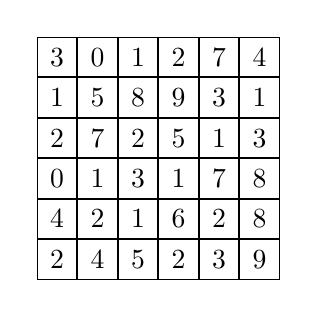
\begin{tikzpicture}
\matrix (m) [matrix of nodes, nodes={draw, inner sep=0pt,text width=0.5cm,align=center,minimum height=0.5cm}]{
3 & 0 & 1 & 2 & 7 & 4\\
1 & 5 & 8 & 9 & 3 & 1\\
2 & 7 & 2 & 5 & 1 & 3\\
0 & 1 & 3 & 1 & 7 & 8\\
4 & 2 & 1 & 6 & 2 & 8\\
2 & 4 & 5 & 2 & 3 & 9\\};
\end{tikzpicture}
\end{figure}
Suppose the above $6\times 6$ matrix is a small grayscale image in which we are trying to detect vertical edges. We use the following convolutional filter for the purpose of vertical edge detection:
\begin{figure}[H]
\centering
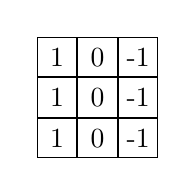
\begin{tikzpicture}
\matrix (m) [matrix of nodes, nodes={draw, inner sep=0pt,text width=0.5cm,align=center,minimum height=0.5cm}]{
1 & 0 & -1\\
1 & 0 & -1\\
1 & 0 & -1\\};
\end{tikzpicture}
\end{figure}
To obtain a matrix representing the vertical edges in the image, we convolve the filter over the image. The convolution operation superimposes the filter on different parts of the image, and creates a matrix of the weighted sums of the overlapping area of the image in each superposition. (The filter matrix acts as weights.) Thus, the convolution operation in this case gives:
\begin{figure}[H]
\centering
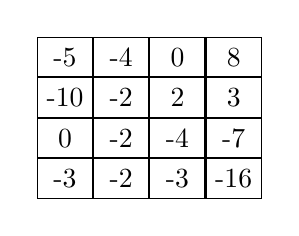
\begin{tikzpicture}
\matrix (m) [matrix of nodes, nodes={draw, inner sep=0pt,text width=0.7cm,align=center,minimum height=0.5cm}]{
-5 & -4 & 0 & 8\\
-10 & -2 & 2 & 3\\
0 & -2 & -4 & -7\\
-3 & -2 & -3 & -16\\};
\end{tikzpicture}
\end{figure}
In this result, the whiter pixels (cells having higher pixel values) are the vertical edges detected by the convolutional operation. This can be understood better by convolving over the following matrix:
\begin{figure}[H]
\centering
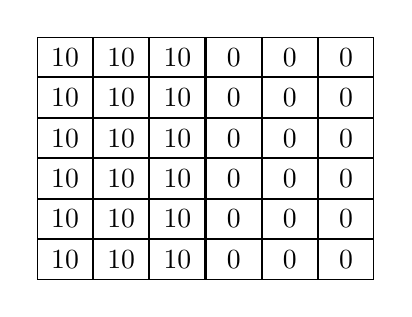
\begin{tikzpicture}
\matrix (m) [matrix of nodes, nodes={draw, inner sep=0pt,text width=0.7cm,align=center,minimum height=0.5cm}]{
10 & 10 & 10 & 0 & 0 & 0\\
10 & 10 & 10 & 0 & 0 & 0\\
10 & 10 & 10 & 0 & 0 & 0\\
10 & 10 & 10 & 0 & 0 & 0\\
10 & 10 & 10 & 0 & 0 & 0\\
10 & 10 & 10 & 0 & 0 & 0\\};
\end{tikzpicture}
\end{figure}
Convolving the vertical edge detector on this gives us:
\begin{figure}[H]
\centering
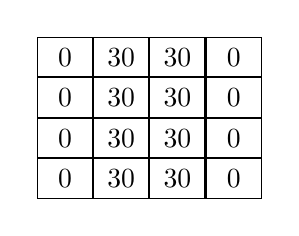
\begin{tikzpicture}
\matrix (m) [matrix of nodes, nodes={draw, inner sep=0pt,text width=0.7cm,align=center,minimum height=0.5cm}]{
0 & 30 & 30 & 0\\
0 & 30 & 30 & 0\\
0 & 30 & 30 & 0\\
0 & 30 & 30 & 0\\};
\end{tikzpicture}
\end{figure}
As we can clearly see, the detector detects an edge along the central vertical region, and we know that to be true from the image itself. This gives us some intuition on the convolution operation.

\section{Padding and Strides}
The result of a convolution (if done as shown above) is smaller in size than the original image. Convolving an $f\times f$ filter over an $n\times n$ image results in an image of size $(n-f+1) \times (n-f+1)$. But often, we may want a result of the same size. To achieve this, we use padding.\\
\break
In the padding technique, we pad the original image to make it larger, by filling in new pixels outside its border (the value is usually zero). The additional thickness (number of border layers added) is called the padding $p$. To achieve a result of the same size as the image, we use the value of padding $p=\dfrac{f-1}{2}$ (because $n+2p-f+1=n$). Note that here we are assuming the convolutional filter to have odd size, which is usually the case. We cannot achieve `same' padding with an even sized convolutional filter. `Same' padding refers to padding such that the output has the same shape as the input, whereas `valid' padding refers to not padding at all.\\
\break
Sometimes, to save time or to achieve some specific purpose, we may not want to superimpose the convolutional filter in every possible place on the image. In that case, we use strided convolutions, where we slide the convolutional filter by some stride length $s$ (in both horizontal and vertical directions) each time before writing the weighted sum into the result. The original case discussed before corresponds to stride $s=1$.

\section{Convolutions over Volume}
In handling images with multiple channels (like RGB or HSV images) in our neural network, we have to convolve filters over volumes. In this technique, we convolve a filter with multiple channels (channels in filter $=$ channels in image) onto the image and obtain a two-dimensional result by convolution. For example:
\begin{figure}[H]
\centering
\includegraphics[width=0.6\textwidth]{conv_volume}
\caption{Convolution over a volume.}
\end{figure}
It's still just like before, only with 3D filters. Also, we may often convolve multiple filters over the image (like if we want to detect both vertical and horizontal edges). Suppose we have an image of shape $n\times n\times n_c$, and we convolve $n'_c$ filters of shape $f\times f\times n_c$ over the image. Then, the result would have the shape $(n-f+1)\times(n-f+1)\times n'_c$.\\
\break
In a way, this is exactly what a convolutional layer does in a neural network. Taking the activations of the previous layer, in the form of a 3D matrix, the convolutional layer convolves several filters over the volume (the filter weights are learned through gradient descent) and passes them on to the activation function in the form of another 3D matrix.

\section{Pooling Layers}
A pooling layer is quite similar to convolution, but in this case, we do not output filter-weighted sums of input values. In pooling layers, we output the maximum (max-pooling) or average (average pooling) value of the values overlapping with the filter. Here, we have an input of size $n\times n\times n_c$, a filter of size $f\times f$, padding $p$, and stride $s$. Then, the output shape of the pooling layer is going to be $\left\lfloor{\dfrac{n+2p-f}{s}+1}\right\rfloor \times \left\lfloor{\dfrac{n+2p-f}{s}+1}\right\rfloor \times n_c$.\\
\break
Note that there are no parameters to be learned in pooling layers. The backpropagation algorithm simply passes through this layer to its previous layers during gradient descent. In a CNN, convolutional layers are almost always followed by max-pooling layers.
\begin{figure}[H]
\centering
\includegraphics[width=0.6\textwidth]{max_pooling}
\caption{An example of a max-pooling layer.}
\end{figure}
An example of a complete CNN, with convolutional layers and max-pooling layers, and fully connected layers at the end, is shown here:
\begin{figure}[H]
\centering
\includegraphics[width=1\textwidth]{cnn_example}
\caption{An example of a complete CNN.}
\end{figure}
This CNN takes as input a hand-written digits (from the MNIST dataset), and classifies it as a digit from 0 to 9. There are two pairs of convolutional and max-pooling layers, followed by two fully-connected (or dense) layers. As we can see, the CNN goes on decreasing the width and height of the data and increasing the number of channels, before finally flattening it out into a 1D array. This technique, used by CNNs, enables them to detect and classify things regardless of which part of the image they appear in.

\section{Why Convolutions?}
There are two main incentives for using convolutions:
\begin{enumerate}
\item Parameter Sharing: In the convolution operation, we move the same filter (of parameters) over the entire data (from the previous layer), and thus we use the same parameters over and over again. Thus, convolution works on the basis that a feature detector that is useful in one part of an image may be useful elsewhere too.
\item Sparsity of Connections: In a convolutional layer, each output value depends on only a small part of the input. Thus, convolutional layers are able to break down an image and analyze its parts independently.
\end{enumerate}
Since computer vision tasks may have the target object in any arbitrary part of the image, convolutions are able to do quite well in such tasks, thanks to the above two characteristics.


\chapter{CNN Architectures}

\section{The LeNet-5 Network Architecture}
The LeNet-5, a classic CNN, has the following architecture:
\begin{figure}[H]
\centering
\includegraphics[width=1\textwidth]{lenet-5}
\caption{The LeNet-5 architecture.}
\end{figure}
The diagram shows its working on the MNIST dataset. There are two convolutional layers, two average-pooling layers, and two fully connected layers. It is clearly quite similar to Figure 14.3. It turns out that the LeNet-5 has close to 60 thousand parameters.

\section{The AlexNet Network Architecture}
The AlexNet, another classic CNN, has the following architecture:
\begin{figure}[H]
\centering
\includegraphics[width=1\textwidth]{alexnet}
\caption{The AlexNet architecture.}
\end{figure}
AlexNet is quite similar to LeNet-5, just a lot bigger. AlexNet has close to 60 million parameters. Note that the original AlexNet had some other layers too, called Local Response Normalization (LRN) layers, which normalized all the channel values at each $x$ and $y$. This was later found to be not very useful, so these layers have been left out.

\section{The VGG-16 Network Architecture}
Yet another classical CNN, called the VGG-16, has the following architecture:
\begin{figure}[H]
\centering
\includegraphics[width=1\textwidth]{vgg}
\caption{The VGG-16 architecture.}
\end{figure}
This also has a similar architecture to the networks above, but even larger. The VGG-16 network has nearly 138 million parameters.

\section{Residual Networks}
Residual networks, also called ResNets, differ from classical CNN architectures in that they are made up of residual blocks. Residual blocks were designed as a solution for the problem of vanishing or exploding gradients in very deep neural networks. A residual block looks like this:
\begin{figure}[H]
\centering
\includegraphics[width=0.5\textwidth]{residual_block}
\caption{Diagram of a residual block.}
\end{figure}
Basically, in a residual block, we have:
\begin{align*}
z^{[l+1]} &= W^{[l+1]}a^{[l]} + b^{[l+1]}\\
a^{[l+1]} &= g(z^{[l+1]})\\
z^{[l+2]} &= W^{[l+2]}a^{[l+1]} + b^{[l+2]}\\
a^{[l+2]} &= g(z^{[l+2]} + W_sa^{[l]})
\end{align*}
Here, $W_s$ is an additional trainable parameter matrix for the skip connection. The main flow in Figure 15.4 is called the main path, whereas the side path is called the skip connection. Skip connections allow activations of a layer to pass to another layer deeper in the network, and thus, due to shorter paths, exploding/vanishing gradients are avoided. A ResNet looks like this:
\begin{figure}[H]
\centering
\includegraphics[width=1\textwidth]{resnet}
\caption{Diagram of a residual network.}
\end{figure}

\section{Inception Networks}
An inception network combines different kinds of convolutions for a single layer of a network. In a single transition from one layer to another, several different kinds of operations are performed (with `same' padding to ensure that the results have the same width and height), such as convolution with a number of $1\times 1$, $3\times 3$, $5\times 5$ filters, as well as pooling filters. All the results are concatenated together along the depth dimension before passing them on to the next layer.\\
\break
However, there is one drawback of the above technique; the computational cost is very high this way. Making each layer's computations more complex would result in inefficient models. To solve this problem, we use a $1\times 1$ convolution over the activations of the previous layer, to squeeze down the data, before applying a $3\times 3$ or a $5\times 5$ convolution.\\
\break
We can understand this through an example. Suppose we have activations of size $28\times 28\times 192$. To get a result of size $28\times 28\times 32$, we apply 32 filters of size $5\times 5\times 192$ with `same' padding. The number of computations we have in this case is $(5\times 5\times 192)\times (28\times 28\times 32)\approx 120$ million. On the other hand, if we first convolve 16 filters of size $1\times 1\times 192$ over the activations, and then convolve 32 filters of size $5\times 5\times 16$ on that, the number of computations we must do is $(1\times 1\times 192)\times(28\times 28\times 16)+(5\times 5\times 16)\times(28\times 28\times 32)\approx 12.4$ million. Thus we see a drastic improvement in computational efficiency with this trick.\\
\break
An inception module thus looks like this:
\begin{figure}[H]
\centering
\includegraphics[width=0.7\textwidth]{inception_block}
\caption{Diagram of an inception block.}
\end{figure}
Note that the $1\times 1$ convolution after max pooling is for the purpose of decreasing the depth of the outcome of max pooling, because this outcome would be as deep as the previous layer activations, and a lot deeper than the outcomes of other convolutions in the inception block. A complete inception network looks like this:
\begin{figure}[H]
\centering
\includegraphics[width=1\textwidth]{inception_network}
\caption{Diagram of an inception network.}
\end{figure}

\chapter{Object Detection and Localization}

\section{Object Localization}
An object localization task comprises checking images for the presence of one out of several objects, identifying the object if present, and drawing a bounding box around it.\\
\break
For an object localization task involving $n$ objects, the target labels are defined as follows:
\begin{align*}
y=
\begin{bmatrix}
p_c\\b_x\\b_y\\b_h\\b_w\\c_1\\c_2\\\vdots\\c_n
\end{bmatrix}
\begin{matrix*}[l]
\rightarrow\text{1 if there is any object in the image, otherwise 0}\\
\rightarrow\text{$x$-coordinate of center of bounding box of the object}\\
\rightarrow\text{$y$-coordinate of center of bounding box of the object}\\
\rightarrow\text{height of bounding box of the object}\\
\rightarrow\text{width of bounding box of the object}\\
\rightarrow\text{1 if the object detected is object no. 1, otherwise 0}\\
\rightarrow\text{1 if the object detected is object no. 2, otherwise 0}\\
\\
\rightarrow\text{1 if the object detected is object no. $n$, otherwise 0}
\end{matrix*}
\end{align*}
If $p_c$ in the above matrix becomes zero, then the rest of the values become ``don't cares". One possible loss metric that can be used for optimization in this task is the mean squared error.
\begin{figure}[H]
\centering
\includegraphics[width=1\textwidth]{object_localization}
\caption{Object localization of a car.}
\end{figure}

\section{Object Detection}
An object detection task consists of checking images for the presence of one or more objects, and drawing bounding boxes around all detected objects. For example, an object detection task for a self-driving car might involve checking images for cars and drawing a bounding box around all the cars detected in every image. Object detection differs from object localization in that, in object detection, there may be several cars in a single image and we now have to detect all of them. For this reason, the localization technique described previously wouldn't work here.
\begin{figure}[H]
\centering
\includegraphics[width=0.6\textwidth]{object_detection}
\caption{Object detection of cars.}
\end{figure}
The most basic object detection algorithm is sliding windows detection. We first train a CNN-based image classifier on close-up images of cars, to predict whether an image is a car or not. Then, we slide a window of a particular size over our image (with some stride in the $x$ and $y$ directions), classifying each resulting image (the part inside the window) as being a car or not, using our CNN. If we get a sufficiently high probability, we use that window position as a bounding box for the car. We have to keep repeating this for a few different window sizes too. Clearly, this has high computational cost with CNNs, making this direct technique practically infeasible.

\section{Convolutional Implementation of Sliding Windows}
The following implementation aims to avoid the computational cost incurred if we pass lots of images (obtained from the window) one by one to our classifier, and just get it over with at once. We just directly pass our entire image into the following CNN.
\begin{figure}[H]
\centering
\includegraphics[width=1\textwidth]{cnn_sliding_windows}
\caption{Sliding windows implementation using CNN.}
\end{figure}
With this technique, we're actually able to perform all the sliding windows classifications in exactly one forward pass. In the figure, we have a $16\times 16\times 3$ image, and we are trying object detection with a $14\times 14$ window, with a stride of 2. The blue square in the initial image shows the part of the image captured by the window's first position, and the blue square in subsequent layers shows the result that would have been obtained if the window part of the image had been passed through a classifier by itself. In this case, we're trying to detect 4 different objects in the image, so the final layer activations have a depth of 4. As we can see, the window's initial position yields a flat layer of depth 4 in the final layer, and similarly, the window's other positions also yield flat layers of the same depth. In this way, we carry out all the window classifications together, saving lots of computational time.

\section{The YOLO Object Detection Algorithm}
YOLO stands for `You Only Look Once'. This algorithm is a state-of-the-art technique for object detection, and it consists of several steps.

\subsection{Labeling the Data}
For the YOLO algorithm, the process of labeling images is slightly complicated.\\
\break
Suppose the object detection task involves $c$ image classes. First, we divide all the images into grids, say $n\times n$. (For example, $n=19$.) To each grid cell, we then assign a number of anchor boxes (say $a$), having different aspect ratios and scales (decided by analyzing the dataset), so as to be able to detect multiple objects centered on the same grid cell. Then, the target label for any input image is defined to be a 3D array of shape $n\times n\times (a\times (5+c))$. To obtain the appropriate values for the label of a particular grid cell, we take all the objects whose centers appear in that grid cell, and we check the IoU values of each of these objects with all the anchor boxes of that grid cell. We pick the anchor box with the highest IoU value as the correct anchor box (we have to pick a unique anchor box for every object centered on that grid cell), and then we fill out the label for that grid cell according to the anchor box selection.\\
\break
IoU (Intersection over Union) of two boxes is defined as the area of their intersection divided by the area of their union. This quantity is used as a measure of similarity between two boxes. By comparing the object's actual bounding box with the anchor boxes of its grid cell, using the IoU measure, we pick which anchor box is most similar in shape to the object's box.
\begin{figure}[H]
\centering
\includegraphics[width=0.3\textwidth]{iou}
\caption{Intersection over union.}
\end{figure}
For example, suppose we have a $3\times 3$ grid (just for simplicity; this is practically very bad), $2$ anchor boxes for each grid (one wider and one taller, for instance), and $3$ object classes (say pedestrians, cars, and bikes). Then, each image label would have a shape $3\times 3\times 16$. Each of the $16$-length sublabels of this label (each lying along the depth dimension) corresponds to a grid cell in the image. Each sublabel (label for a grid cell) is of this form:
\begin{align*}
y=
\begin{bmatrix}
p_c\\b_x\\b_y\\b_h\\b_w\\c_1\\c_2\\c_3\\p_c\\b_x\\b_y\\b_h\\b_w\\c_1\\c_2\\c_3
\end{bmatrix}
\begin{matrix*}[l]
\rightarrow\text{1 if it has an object overlapping best with $1^{\text{st}}$ anchor box, otherwise 0}\\
\rightarrow\text{$x$-coordinate of center of bounding box of the object with anchor box 1}\\
\rightarrow\text{$y$-coordinate of center of bounding box of the object with anchor box 1}\\
\rightarrow\text{height of bounding box of the object with anchor box 1}\\
\rightarrow\text{width of bounding box of the object with anchor box 1}\\
\rightarrow\text{1 if the object detected is object no. 1, otherwise 0}\\
\rightarrow\text{1 if the object detected is object no. 2, otherwise 0}\\
\rightarrow\text{1 if the object detected is object no. 3, otherwise 0}\\
\rightarrow\text{1 if it has an object overlapping best with $2^{\text{nd}}$ anchor box, otherwise 0}\\
\rightarrow\text{$x$-coordinate of center of bounding box of the object with anchor box 2}\\
\rightarrow\text{$y$-coordinate of center of bounding box of the object with anchor box 2}\\
\rightarrow\text{height of bounding box of the object with anchor box 2}\\
\rightarrow\text{width of bounding box of the object with anchor box 2}\\
\rightarrow\text{1 if the object detected is object no. 1, otherwise 0}\\
\rightarrow\text{1 if the object detected is object no. 2, otherwise 0}\\
\rightarrow\text{1 if the object detected is object no. 3, otherwise 0}
\end{matrix*}
\end{align*}

\subsection{Neural Network}
A convolutional neural network is then designed, with the images (in which objects are to be detected) as the input and the labels defined above as the desired output. We train this convolutional neural network as we would train any other.

\subsection{Non-max Suppression}
Before making the final object detection predictions, we apply non-max suppression on the output of the convolutional neural network. This step is important because, for an object spanning several grid cells (which is usually the case), many of these grid cells are likely to think that they have found the object, and since all of them work independently in this algorithm, several bounding boxes are going to be predicted for each object. Also, some bounding boxes may have very low probability of containing an object, so we need to deal with that too.\\
\break
So first of all, we get rid of all bounding boxes that have object probabilities less than some threshold (say 0.4). Next, we find the bounding box with the highest probability for object class 1. We check the IoU value of this box with all the other boxes of object class 1, and we get rid of those boxes which have IoU greater than 0.5 (or some other appropriate threshold) with this maximum probability box. Now, we check the remaining boxes (leaving out the max one) for the highest probability of class 1, and then eliminate class 1 boxes having high IoU with that box, and so on. Ultimately, we end up with just one box (probably) for every object of class 1 in the image. We now repeat the same process for every class. Thus, the non-max suppression technique basically checks all the boxes detecting a particular class to find which boxes are detecting the same object, selects the highest probability box out of these, and gets rid of the rest.

\chapter{Face Recognition and One-Shot Learning}

\section{Verification versus Recognition}
A face verification task comprises comparing an input image of a person with another image of a person (stored previously), to predict whether they are of the same person.\\
\break
On the other hand, a face recognition task on a database of $K$ people involves performing $K$ face verification tasks, i.e., comparing the input image with all $K$ images of people to decide if it is one of them, and if yes, then who it actually is.\\
\break
One major difference in face verification/detection tasks from other learning tasks is that we have only one or a few images of people. For example, a company wouldn't have a large dataset of each of its employees' images. This is where one-shot learning comes in; we have to predict whether two images are of the same person using just one pair of images. So, this is what every face verification and recognition problem finally boils down to; detecting similarity of images.

\section{One Shot Learning Approach}
Clearly, because we have just one image (or very few images) per class (each class is a person in this case), training a CNN-based classifier to classify images to people is going to be a very very bad idea. This would never work out. So we adopt a different approach for one-shot learning.\\
\break
To measure similarity between images, we train a similarity function. For example, suppose we train and obtain a function d(img1,img2), which is a measure of the difference between img1 and img2. We use some threshold value $\tau$, and we say that the images are of the same person if d(img1,img2) $\leq\tau$, and we say they are of different people if d(img1,img2) $>\tau$.

\section{Siamese Network}
A Siamese network architecture is used for the face verification task. In this task, the motive is to take two images and measure the similarity between them. So, in a Siamese network, each image is passed through a convolutional neural network (the same for both) which outputs a flattened feature vector of some predetermined dimension. With the two output vectors $f(x^{(1)})$ and $f(x^{(2)})$, we calculate the distance between the images, $\lVert f(x^{(1)})-f(x^{(2)})\rVert^2$. We finally use this distance as the difference function between the images. We train our Siamese network on some training dataset so that it predicts lower difference values for images of the same person and higher difference values for images of different people.
\begin{figure}[H]
\centering
\includegraphics[width=0.6\textwidth]{siamese_network}
\caption{A Siamese network architecture.}
\end{figure}

\section{Triplet Loss}
How exactly do we train a Siamese network? We already have our output label definition, and we have our neural network. But we still don't have a loss function. We use the triplet loss function for our network.\\
\break
In the triplet loss (contrastive loss) function, we take one anchor image $A$ of any random person, one positive image $P$ of the same person, and one negative image $N$ of a different person. We perform the forward pass for the image pairs $(A,P)$ and $(A,N)$, computing the difference function for each pair. So, now we have $\lVert f(A)-f(P)\rVert^2$ and $\lVert f(A)-f(N)\rVert^2$. For an ideal network, we would want the former to be quite a bit smaller than the latter. So, using a hyperparameter $\alpha$, we can write our objective as:
\begin{align*}
\lVert f(A)-f(P)\rVert^2 + \alpha \leq \lVert f(A)-f(N)\rVert^2
\end{align*}
If this is achieved for some triplet $(A,P,N)$, then we aren't worried at all. If not, we impose a cost. Thus, we define our loss function for a particular triplet as follows:
\begin{align*}
L(A,P,N)=\max\left(\lVert f(A)-f(P)\rVert^2 - \lVert f(A)-f(N)\rVert^2 + \alpha, 0\right)
\end{align*}
We compute our cost function by averaging our losses over a mini-batch of samples, and then we use gradient descent (as usual) to make our weights better.\\
\break
Note that an alternative for the triplet loss method is to extend the Siamese network, combining the two vectors to obtain a final sigmoid unit, which outputs 1 for same person and 0 for different people. This way, we can convert our problem into binary classification.

\chapter{Neural Style Transfer}

\section{What is NST?}
Neural style transfer (NST) is a cool technique used to recreate a picture in the style of some other image, maybe a painting by some artist.
\begin{figure}[H]
\centering
\includegraphics[width=1\textwidth]{nst}
\caption{An example of neural style transfer.}
\end{figure}
In neural style transfer, the picture to be recreated (which supplies the `content' of our output) is called the content image $C$, whereas the picture whose style is to be used (which supplies the `style' of our output) is called the style image $S$. The final output image is called the generated image $G$.

\section{Cost Function}
To implement NST, we first create a random image (initialized with random pixel values), and then we make it better through gradient descent. For this purpose, we need a cost function. We define the cost function as follows:
\begin{align*}
J(G) = \alpha J_{\text{content}}(C,G) + \beta J_{\text{style}}(S,G)
\end{align*}
Here, $\alpha$ and $\beta$ are hyperparameters of our model, which can be tweaked to make the generated image closer to either the content image or the style image.

\subsection{Content Cost Function}
Select an intermediate hidden layer $l$ of the CNN, for computing the content cost. (Using a pre-trained CNN gives pretty good results.) Let $a^{[l](C)}$ and $a^{[l](G)}$ be the activations of layer $l$ for the content image and generated image respectively. Then, the content cost is defined as:
\begin{align*}
J_{\text{content}}(C,G) = \dfrac{1}{2}\lVert a^{[l](C)}-a^{[l](G)}\rVert^2
\end{align*}

\subsection{Style Cost Function}
We first define some additional hyperparameters $\lambda^{[l]}$, to determine the weights we give to each layer of the network. Then, we can define our style cost function as follows:
\begin{align*}
J_{\text{style}}(S,G) = \sum_{l}\lambda^{[l]}J_{\text{style}}^{[l]}(S,G)
\end{align*}
Here, $J_{\text{style}}^{[l]}(S,G)$ is defined as:
\begin{align*}
J_{\text{style}}^{[l]}(S,G) = \dfrac{1}{\left(2n_H^{[l]}n_W^{[l]}n_C^{[l]}\right)^2}\sum_{k}\sum_{k'}\left(G_{kk'}^{[l](S)}-G_{kk'}^{[l](G)}\right)^2
\end{align*}
In this equation, $G_{kk'}^{[l](S)}$ and $G_{kk'}^{[l][G]}$ are called Gram matrices. They are defined as follows:
\begin{align*}
G_{kk'}^{[l](S)} &= \sum_{i=1}^{n_H^{[l]}}\sum_{j=1}^{n_W^{[l]}}a_{ijk}^{[l](S)}a_{ijk'}^{[l](S)}\\
G_{kk'}^{[l](G)} &= \sum_{i=1}^{n_H^{[l]}}\sum_{j=1}^{n_W^{[l]}}a_{ijk}^{[l](G)}a_{ijk'}^{[l](G)}
\end{align*}
The Gram matrix is a measure of the correlations between different channels of activations in a layer of the network.

\chapter{Recurrent Neural Networks (RNNs)}

\section{Why do we need Sequence Models?}
So far, we have only worked with data where we do not need to bother with whether something occurs earlier or later in the data. But we cannot deal with all learning tasks this way; for example, making a transcription for a voice recording involves the time dimension, as the words need to be arranged in the order in which they were spoken. Similarly, in the analysis of a DNA sequence, it is important to observe the order in which nucleotides occur in the sequence. For such cases, we need a new type of neural network architecture; the previous ordinary networks and CNNs cannot deal with sequence data appropriately. This is why we need sequence models.

\section{Notation}
A new kind of notation is used for sequence models.
\begin{enumerate}
\item We use $x^{(i)<t>}$ to denote the $t^{\text{th}}$ element of the input sequence belonging to the $i^{\text{th}}$ data instance. (The letter $t$ is used to create a notion of time.)
\item Similarly, we use $y^{(i)<t>}$ to denote the $t^{\text{th}}$ element of the output sequence belonging to the $i^{\text{th}}$ data instance.
\item We use $T_{x}^{(i)}$ to denote the length of the input sequence belonging to the $i^{\text{th}}$ data instance.
\item We use $T_{y}^{(i)}$ to denote the length of the output sequence belonging to the $i^{\text{th}}$ data instance.
\end{enumerate}

\section{Basic RNN Architecture}
A typical recurrent neural network looks like this:
\begin{figure}[H]
\centering
\includegraphics[width=0.55\textwidth]{rnn}
\caption{A recurrent neural network (RNN).}
\end{figure}
This is the unrolled form of the RNN; there is a more compact way of representation, but this one is easier to understand. Accompanying the RNN diagram, we have the following equations:
\begin{align*}
a^{<0>} &= 0\\
a^{<t>} &= g\left(W_{aa}a^{<t-1>}+W_{ax}x^{<t>}+b_{a}\right)\\
\hat{y}^{<t>} &= g\left(W_{ya}a^{<t>}+b_{y}\right)
\end{align*}
The notation can be simplified as follows:
\begin{align*}
a^{<t>} &= g\left(W_{a}\left[a^{<t-1>}, x^{<t>}\right]+b_{a}\right)\\
\hat{y}^{<t>} &= g\left(W_{y}a^{<t>}+b_{y}\right)
\end{align*}
Here, $W_{a}$ is the matrix obtained by horizontally stacking together the weight matrices $W_{aa}$ and $W_{ax}$, $\left[a^{<t-1>}, x^{<t>}\right]$ is the matrix obtained by vertically stacking together the matrices $a^{<t-1>}$ and $x^{<t>}$, and $W_{y}$ is the same as $W_{ya}$.\\
\break
The loss function for any data instance is as follows:
\begin{align*}
L(\hat{y}, y) = \sum_{t=1}^{T_y}L(\hat{y}^{<t>}, y^{<t>})
\end{align*}
where:
\begin{align*}
L(\hat{y}^{<t>}, y^{<t>}) = -\left(y^{<t>}\log\left(\hat{y}^{<t>}\right) + (1-y^{<t>})\log\left(1-\hat{y}^{<t>}\right)\right)
\end{align*}
As always, we use backpropagation with gradient descent to improve the parameters step by step. The parameters that are trained are $W_a$ and $W_y$.

\section{Types of RNNs}
Different types of RNNs, on the basis of number of inputs and number of outputs, are:
\begin{figure}[H]
\centering
\includegraphics[width=0.8\textwidth]{rnn_types}
\caption{Types of recurrent neural networks.}
\end{figure}
A one-to-one RNN is essentially equivalent to a logistic regression unit.\\
\break
A one-to-many RNN has just one input, and each output after the first is generated by using the previous output as the next input, as shown in figure. An example where this is used is in image captioning, where we input a single image and generate an appropriate sentence using sequence output.\\
\break
A many-to-one RNN has a sequence input and a single output after the last input. An example where this is used is sentiment classification, where we input one or more sentences as sequence input and we output whether the emotions being conveyed are positive or negative.\\
\break
A many-to-many RNN may be of two different types. The first one in the diagram is used when $T_x = T_y$, i.e., each element of the input sequence has a corresponding element in the output sequence. For example, this is used when, given a sentence, we want to identify the names in it. We would output 1 for name words, and 0 for other words. The second one in the diagram is used in cases where there is no element-to-element correspondence between the input and the output. So, all the output is generated only after the entire input sequence has been processed. An example where this is used is in machine translation, such as from English to French.

\section{Language Models}
A language model is used to compare probabilities of two sentences. This basically means, if someone speaks any sentence randomly, what is the likelihood that he/she speaks a particular sentence? We calculate the probabilities of both sentences and compare. This is useful in speech recognition and transcription systems, to compare the likelihoods of several sentences that are possible transcriptions. (This enables systems to choose between homophones, like pair and pear.)\\
\break
To calculate the probability of a sentence being spoken randomly, we first find a way to represent sentences as sequences for RNNs. We thus create a dictionary of all possible words that we can come across, using one index for each word. Then, we represent each word using a one-hot encoding, where the element which corresponds to word's index in the dictionary has value 1 and all others have 0. Note that we should also give a place in the dictionary to `end of sentence' (EOS) and to unknown words (UNK).\\
\break
To create a language model, we use a many-to-many RNN as shown here:
\begin{figure}[H]
\centering
\includegraphics[width=0.8\textwidth]{language_model}
\caption{A language model architecture.}
\end{figure}
In a language model, the first input element is a zero. So as our first output, we generate a vector containing the probabilities of every possible word for occurring as the first word of a sentence. For our second input, we give the actual first word of the sentence, and output the probabilities of every possible word for occurring as the second word of a sentence that begins with the real first word. Thus, we have that $\hat{y}^{<t>}$ is the vector of probabilities of words occurring at the $t^{\text{th}}$ position of the sentence given the previous $t-1$ words of the sentence. For example, consider the sentence ``I want some pear salad." In this case, $\hat{y}^{<4>}$ is the vector of probabilities for the next word in the sentence given the first three words are ``I want some". When we reach the end of the sentence, we calculate the probability of the sentence as:
\begin{align*}
P(y^{<1>},\dots,y^{<T_y>}) = P(y^{<1>})\cdot P(y^{<2>}|y^{<1>})\cdot P(y^{<3>}|y^{<1>},y^{<2>})\cdots P(y^{<T_y>}|y^{<1>},\dots,y^{<T_y-1>})
\end{align*}
A language model can be trained on a large text corpus using the same loss function as discussed above in general RNNs.

\section{Novel Sequence Sampling}
Sampling novel sequences involves getting random meaningful sequence outputs from a language model. For example, we can use this technique to generate random sentences. The language model is first trained (as already discussed). Then, the value of $x^{<1>}$ is passed in as 0. As the first word, we select any word randomly, but we use the probabilities output in $y^{<1>}$ for the word selection. We then pass in the selected first word as the second input, and this process goes on until the end. This generates a random sentence.\\
\break
Note that, if we select the highest probability words from the output vectors, instead of choosing words randomly with the output probabilities as we did, we would always end up with the same output sentence. So that doesn't work out.

\section{Gated Recurrent Units (GRUs)}
Just like other neural networks, RNNs also suffer from the problems of vanishing and exploding gradients. While exploding gradients can be cured through gradient clipping (any gradient values too large in magnitude are clipped to a maximum limit), it requires a little more effort to solve the vanishing gradient problem. Using GRUs instead of ordinary RNN units is one way.
\begin{figure}[H]
\centering
\includegraphics[width=0.45\textwidth]{rnn_unit}
\caption{An RNN unit.}
\end{figure}
We can represent an ordinary RNN unit as shown above. (We've considered the tanh activation function here.) In a similar way, a gated recurrent unit can be represented as follows:
\begin{figure}[H]
\centering
\includegraphics[width=0.7\textwidth]{gru}
\caption{A gated recurrent unit.}
\end{figure}
Here, we have replaced $a^{<t>}$ with $h^{<t>}$. The equations in play here are:
\begin{align*}
r^{<t>} &= \sigma\left(W_r\left[h^{<t-1>}, x^{<t>}\right] + b_r\right)\\
z^{<t>} &= \sigma\left(W_z\left[h^{<t-1>}, x^{<t>}\right] + b_z\right)\\
\hat{h}^{<t>} &= \text{tanh}\left(W_h\left[r^{<t>}*h^{<t-1>}, x^{<t>}\right] + b_h\right)\\
h^{<t>} &= z^{<t>}*\hat{h}^{<t>} + \left(1-z^{<t>}\right)*h^{<t-1>}
\end{align*}
This way, we can use a weighted sum of the previous activation and the result of the current layer to calculate the current layer activation, and this helps avoid the vanishing gradients problem.

\section{Long Short Term Memory (LSTM)}
LSTM units are another way to deal with sequence learning tasks. These are more widely used than GRUs or ordinary RNNs. An LSTM unit is represented as follows:
\begin{figure}[H]
\centering
\includegraphics[width=0.6\textwidth]{lstm_unit}
\caption{An LSTM unit.}
\end{figure}
In LSTM units, we keep two kinds of values, $a^{<t>}$ and $c^{<t>}$. The math is as follows:
\begin{align*}
\tilde{c}^{<t>} &= \text{tanh}\left(W_c\left[a^{<t-1>}, x^{<t>}\right] + b_c\right)\\
\Gamma_u &= \sigma\left(W_u\left[a^{<t-1>}, x^{<t>}\right] + b_u\right)\\
\Gamma_f &= \sigma\left(W_f\left[a^{<t-1>}, x^{<t>}\right] + b_f\right)\\
\Gamma_o &= \sigma\left(W_o\left[a^{<t-1>}, x^{<t>}\right] + b_o\right)\\
c^{<t>} &= \Gamma_u*\tilde{c}^{<t>} + \Gamma_f*c^{<t-1>}\\
a^{<t>} &= \Gamma_o*\text{tanh}\left(c^{<t>}\right)
\end{align*}
LSTM units have been found to deal very effectively with sequence tasks, and vanishing gradients are encountered much less frequently when using LSTMs.

\section{Bidirectional RNNs}
Often, in sequence learning tasks, it is useful to consider the entire input sequence when producing any outputs. In case this is true, and $T_x = T_y$, we prefer using bidirectional RNNs over the second kind of many-to-many RNNs (see figure 19.2). In bidirectional RNNs, we have the sequence running in both directions, as shown:
\begin{figure}[H]
\centering
\includegraphics[width=0.6\textwidth]{bidirectional_rnn}
\caption{A bidirectional recurrent neural network.}
\end{figure}


\chapter{Word Representations}

\section{Word Embeddings}
So far, we have used simple one-hot encoded word representations, based on a dictionary. This is not good enough; for example, suppose the RNN has learned that the word `juice' is a very probable next word after the words ``I want a glass of apple". It would be very good if the model recognized apple and orange as similar things (both fruits), so that it would predict `juice' after the words ``I want a glass of orange" as well. To achieve this, we use word embeddings.\\
\break
Word embeddings are featurized word representations, i.e., the $i^{\text{th}}$ element of the embedding for each word represents the relation of the word to some feature. For example, if the feature was `fruit', both apple and orange would have high values. In practice, these features may not represent something humanly understandable (like `fruit'), since they are learned by the model.\\
\break
If we use word embeddings, then the features are learned so that the vectors representing similar words occur close to each other in the multidimensional space of features. Similar word embeddings of words helps the model recognize similar words, and thus work better. Word embeddings can be learnt on a large text corpus (or we could just use already available word embeddings), and then used (like transfer learning) for the task at hand.

\section{Analogies in Word Embeddings}
Word embeddings also contain analogies, which turn out to be useful for certain tasks. For example, through its feature vectors, a word embedding can solve questions like: man $\rightarrow$ woman as king $\rightarrow$ ?, for which the answer is obviously queen. For example, consider this (oversimplified) word embedding:
\begin{figure}[H]
\centering
\includegraphics[width=0.7\textwidth]{analogies}
\caption{A word embedding.}
\end{figure}
We analyze how we can solve the same problem: find X if man $\rightarrow$ woman as king $\rightarrow$ X. If this analogy holds, then we have: $e_{\text{man}} - e_{\text{woman}} \approx e_{\text{king}} - e_{\text{X}}$. So, we simply calculate the vector $e_{\text{king}} - e_{\text{man}} + e_{\text{woman}}$, and we find the word whose embedding vector is closest to it. This word is our answer. Thus, the answer is:
\begin{align*}
\text{X} = \text{arg}\max_{w}\text{sim}\left(e_w, e_{\text{king}} - e_{\text{man}} + e_{\text{woman}}\right)
\end{align*}
where sim is a similarity function. The cosine similarity function is often used:
\begin{align*}
\text{sim}(u,v) = \dfrac{u^{T}v}{\norm{u}_2\norm{v}_2}
\end{align*}

\section{Word Embedding Matrix}
The embedding matrix $E$ is the matrix consisting of embeddings of all the words in our dictionary. Suppose our vocabulary size is $m$, and we have learnt word embeddings with $n$ features. Then the embedding matrix has shape $n\times m$, with each column representing the word embedding of a single word from our vocabulary.\\
\break
Let $o_k$ be the one-hot encoding of the $k^{\text{th}}$ word in our dictionary. Then, the word embedding for the $k^{\text{th}}$ word would be $E\cdot o_k$. Computationally, though, a word embedding is selected by slicing through the embedding matrix, since matrix multiplication has higher computational costs.

\section{Word2Vec Model}
The Word2Vec model is one method of learning word embeddings. Suppose we have a dictionary of $m$ words, and the embeddings are trained to have $n$ features. To train our embeddings, we first select a word at random from our text corpus, and call it the context word $c$. Then, from some window of a few words (maybe 4-5) surrounding the context word, we select another word at random and call it the target word $t$.\\
\break
To make the context and target words for each such selection have similar word embeddings, we actually work on a different supervised learning problem; given the context word, we try predicting the target word. For this purpose, we feed the context word embedding $e_c = E\cdot o_c$ into a softmax unit. Each word in the dictionary is given a corresponding parameter vector $\theta$, and the calculation done in the softmax unit is:
\begin{align*}
P(t|c) = \dfrac{e^{\theta_t^T e_c}}{\sum_{j=1}^{m}e^{\theta_j^T e_c}}
\end{align*}
This way, the softmax unit uses the parameter vector $\theta$ of every possible target word to calculate its own probability of being the target word. The loss function used is:
\begin{align*}
L(\hat{y}, y) = -\sum_{i=1}^{m}y_i\log(\hat{y}_i)
\end{align*}
where $\hat{y}$ is the vector of probabilities calculated by the softmax unit, and $y$ is the one-hot encoded vector for the actual target word. Using gradient descent with this loss function, we can train pretty good word embeddings.

\section{Negative Sampling}
The Word2Vec technique has very high computational cost, because of the softmax unit. To solve this problem, negative sampling is used. Every time we pick a context word and target word, we also pick a number of negative samples; we actually just pick any $k$ random words in our dictionary, since randomly selected words are still very likely to be unrelated to the context word in case of a good-enough vocabulary.\\
\break
As before, we calculate $e_c$ for the context word, but instead of a softmax unit, we now use a binary classifier for every possible target word, which uses the sigmoid activation function, and outputs $\sigma(\theta_t^T e_c)$. We train the classifier corresponding to the chosen target word with an expected output of 1, and then we train the classifiers corresponding to the $k$ random (assumed negative) samples with expected outputs of 0. We simply ignore the other classifiers (for words other than our $k+1$ chosen words) at this step, and we move on to choose another context word. This way, computational costs are reduced significantly.

\section{GloVe Model}
The global vectors for word representation (GloVe) model is another method of training word embeddings. In this method, we first calculate $X_{ij}$, the number of times $j$ occurs in the context of $i$ in our text corpus, for all $i$ and $j$. Then, the optimization problem is as follows:
\begin{align*}
\min_{\theta, b, e} \sum_{i=1}^{m}\sum_{j=1}^{m}f(X_{ij})\left(\theta_i^T e_j + b_i + b_j' - \log X_{ij}\right)^2
\end{align*}
It is easy to see that $\theta$ and $e$ become totally symmetric in the GloVe model. Thus, the final embedding for any word $w$ is taken as $\dfrac{e_w + \theta_w}{2}$. Also, $f(X_{ij})$ is kept as 0 if $X_{ij}=0$, to zero out the undefined value of $\log(0)$, and it is allowed to have other values for other cases.

\section{Debiasing Word Embeddings}
Being trained on a random text corpus, a word embedding may often suffer from stereotypes. An analogy such as man $\rightarrow$ scientist as woman $\rightarrow$ ? may produce an answer like `homemaker'. Obviously, we would want to remove stereotypes related to gender, race, ethnicity, sexual orientation, etc. from word embeddings.\\
\break
Let us formulate a solution to the gender bias problem. We first find out the approximate direction of gender bias in our word embeddings, by taking the average value of several vectors like $e_{\text{he}}-e_{\text{she}}$, $e_{\text{boy}}-e_{\text{girl}}$, $e_{\text{man}}-e_{\text{woman}}$, $e_{\text{him}}-e_{\text{her}}$, etc. We then find the $n-1$ dimensional hyperplane perpendicular to this direction, which represents the non-gender-bias direction.\\
\break
Next, we project the vector of every non-definitional word (scientist, homemaker, doctor, etc., which should be gender independent) onto the non-gender-bias hyperplane, to get rid of gender biases. But we are not done yet; it may so happen that `he' is still closer to `scientist' than `she', and `she' is closer to homemaker than `he'. To solve this, we also need to equalize the distances of each definitional word (such as `he' and `she') on opposite sides of the non-gender-bias hyperplane.\\
\break
Let $g$ be the vector in the direction of gender bias. Then, for debiasing a non-definitional word, we replace its word embedding $e$ with:
\begin{align*}
e_{\text{debiased}} = e - \dfrac{e\cdot g}{\norm{g}_2^2}*g
\end{align*}
The equalization of pairs of non-definitional words is more complex:
\begin{align*}
\mu &= \dfrac{e_{w1}+e_{w2}}{2}\\
\mu_B &= \dfrac{\mu\cdot g}{\norm{g}_2^2}*g\\
\mu_{\perp} &= \mu - \mu_B\\
e_{w1B} &= \dfrac{e_{w1}\cdot g}{\norm{g}_2^2}*g\\
e_{w2B} &= \dfrac{e_{w2}\cdot g}{\norm{g}_2^2}*g\\
e_{w1B}^{\text{corrected}} &= \sqrt{|1-\norm{\mu_\perp}_2^2|} * \dfrac{e_{w1B}-\mu_B}{\norm{(e_{w1}-\mu_\perp)-\mu_B}}\\
e_{w2B}^{\text{corrected}} &= \sqrt{|1-\norm{\mu_\perp}_2^2|} * \dfrac{e_{w2B}-\mu_B}{\norm{(e_{w2}-\mu_\perp)-\mu_B}}\\
e_1 &= e_{w1B}^{\text{corrected}}+\mu_\perp\\
e_2 &= e_{w2B}^{\text{corrected}}+\mu_\perp
\end{align*}


\chapter{Many-to-Many RNNs}

\section{Machine Translation Model}
The following kind of many-to-many RNN model is used for machine translation:
\begin{figure}[H]
\centering
\includegraphics[width=0.7\textwidth]{machine_translation}
\caption{A many-to-many model for machine translation.}
\end{figure}
This model can be thought of as a conditional language modelling network; it is similar to a language model, but now with some input taken before the sentence generation begins. The sentence generated here is chosen based on $P(y^{<1>},\dots,y^{<T_y>}|x^{<1>},\dots,x^{<T_x>})$. As before, we can use a greedy algorithm, just moving on generating a new word at each step with probabilities decided by the words already chosen.\\
\break
However, there is one drawback to using greedy algorithms; we cannot go back to make changes if we later realize that another beginning to the sentence would have been better. This means the greedy algorithm may not end up with the most probable sentence. To tackle this problem, we use beam search.

\section{Beam Search}
Beam search is similar the greedy algorithm mentioned above; the only difference is that beam search tries to keep several options open, just in case a sentence other than the one produced by the greedy approach turns out to be better.\\
\break
In beam search, we have a beam width $B$, which is the number of options we keep open at each step of next word prediction. The model used is still the one shown in figure 21.1. For the first word prediction, we generate the probability corresponding to every word in our dictionary. Out of these $m$ words, we then pick the $B$ most probable words, and remember them. For the second word prediction, we feed in each of the $B$ words one by one to the next input of the RNN, each time generating probabilities of occurring as the second word, corresponding to all possible words in the dictionary. Out of these $B\cdot m$ options, we then select the $B$ most probable word couples (first and second word pairs), and remember these for the third step. In this way, we keep moving forward, and at the end, we pick the most probable sentence in our beam. The following diagram shows beam search with $B=3$:
\begin{figure}[H]
\centering
\includegraphics[width=0.7\textwidth]{beam_search}
\caption{Beam search with a beam width of 3.}
\end{figure}
Note that the machine translation model is distinctly divided into the RNN component and the beam search component, making error analysis easier. If the algorithm outputs a translation that is not good enough, then we can attribute the mistake to one of the two components by comparing the computed probabilities of the two translations. If the algorithmic translation is not good enough, and yet it had higher probability according to the model, the RNN is at fault. If the probability of the algorithm's translation is less than that of the ideal translation, we can conclude that beam search is at fault.

\section{Sentence Length Normalization}
In these machine translation models, we are calculating:
\begin{align*}
P(y^{<1>},\dots,y^{<T_y>}|x^{<1>},\dots,x^{<T_x>}) = P(y^{<1>}|x)\cdot P(y^{<2>}|x,y^{<1>})\cdots P(y^{<T_y>}|x,y^{<1>},\dots,y^{<T_y-1>})
\end{align*}
But this gives an undesirable probability advantage to shorter output sequences. To solve this problem, we use sentence normalization. Instead of solving:
\begin{align*}
\text{arg}\max_{y} \prod_{t=1}^{T_y} P\left(y^{<t>}|x,y^{<1>},\dots,y^{<t-1>}\right)
\end{align*}
we solve the following optimization problem:
\begin{align*}
\text{arg}\max_{y} \dfrac{1}{T_y^\alpha}\sum_{t=1}^{T_y} \log P\left(y^{<t>}|x,y^{<1>},\dots,y^{<t-1>}\right)
\end{align*}
where $\alpha$ is some hyperparameter between 0 and 1.

\section{Bleu Score}
The bilingual evaluation understudy (Bleu) score is a way to automatically evaluate machine translations. Given a machine translation $\hat{y}$ and a number of human translations, we calculate:
\begin{align*}
\text{Bleu score on n-grams} = p_n = \dfrac{\sum_{\text{n-grams}\in\hat{y}}\text{count}_{\text{clipped}}(\text{n-gram})}{\sum_{\text{n-grams}\in\hat{y}}\text{count}(\text{n-gram})}
\end{align*}
where $\text{count}(\text{n-gram})$ represents the number of times that n-gram appears in the machine translation $\hat{y}$, and $\text{count}_{\text{clipped}}(\text{n-gram})$ represents the maximum number of times that n-gram appears in any one of the human translations.\\
\break
Considering $p_1,p_2,\dots,p_k$, the combined Bleu score is:
\begin{align*}
\text{BP}\cdot\exp\left(\dfrac{1}{k}\sum_{n=1}^{k}p_n\right)
\end{align*}
where BP is called the brevity penalty, and takes a value of 1 if the machine translation is longer than the human translations, and a value of $\exp\left(1-\dfrac{\text{human translation length}}{\text{machine translation length}}\right)$ otherwise.

\section{Attention Models}
Suppose we need to translate a long paragraph from one language to another. Clearly, the many-to-many RNN discussed so far would not be very effective for this task, as it would have to memorize a lot of things all at once before it can start producing output. This is why we need attention models.\\
\break
An attention model looks like this:
\begin{figure}[H]
\centering
\includegraphics[width=0.6\textwidth]{attention_model}
\caption{An attention model.}
\end{figure}
The input sentence is fed into a bidirectional RNN, to encode into feature vectors. Then, the output sentence is produced by another RNN whose inputs are the encoded feature vectors, with each RNN unit having some attention weights corresponding to every encoded feature vector. The parameter $\alpha^{<t,t'>}$ is the attention that $y^{<t>}$ gives to the feature vector produced from $a^{<t'>}$. The attention weights for a particular output add up to one, i.e., $\sum_{t'}\alpha^{<t,t'>}=1$.\\
\break
The attention weights are computed as follows:
\begin{align*}
\alpha^{<t,t'>} = \dfrac{\exp\left(e^{<t,t'>}\right)}{\sum_{t'=1}^{T_x}\exp\left(e^{<t,t'>}\right)}
\end{align*}
This step ensures that the sum of all attention weights for a particular output is 1. The values of $e^{<t,t'>}$ are obtained as output from a simple neural network, having inputs $s^{<t-1>}$ and $a^{<t'>}$.\\
\break
This algorithm produces very good results for translating long sentences, but it takes quadratic time to execute, which may be too heavy for some applications.

\newpage

\topskip0pt
\vspace*{\fill}
\begin{center}
{\huge\scshape End of Report}
\end{center}
\vspace*{\fill}

\end{document}